\documentclass[ignorenonframetext, 10pt, aspectratio=169]{beamer}

\usepackage{preamble_slides}


\title{\textbf{\Large{Git for Students in the Social Sciences$^*$: A Pitch}}}
\providecommand{\subtitle}[1]{}
\subtitle{($^*$ not software developers)}
\author{Shiro Kuriwaki}
\date{\small \textcolor{gray}{Presented March 5, 2019;~~ Last updated \today}}

\begin{document}

\begin{frame}{Setup Today}
\begin{columns}[T]
\begin{column}{0.6\textwidth}
\begin{wideenumerate}
\item Keep  \url{www.happygitwithr.com} open
\item Go to \url{www.github.com} and make a free account
\begin{wideitemize}
\item[-] \textcolor{gray}{\footnotesize Pick a professional, short username; it's hard to change later. More tips at Chapter 4.1 of happygitwithr,  \url{https://happygitwithr.com/github-acct.html\#username-advice}}
\end{wideitemize}
\item Make sure you have a recent version (v1.1 or later) of RStudio \url{https://www.rstudio.com/products/rstudio/download/\#download}
\item Download these slides via the repository: \url{https://bit.ly/2XHXyl1}.
\end{wideenumerate}
\end{column}
\begin{column}{0.4\textwidth}
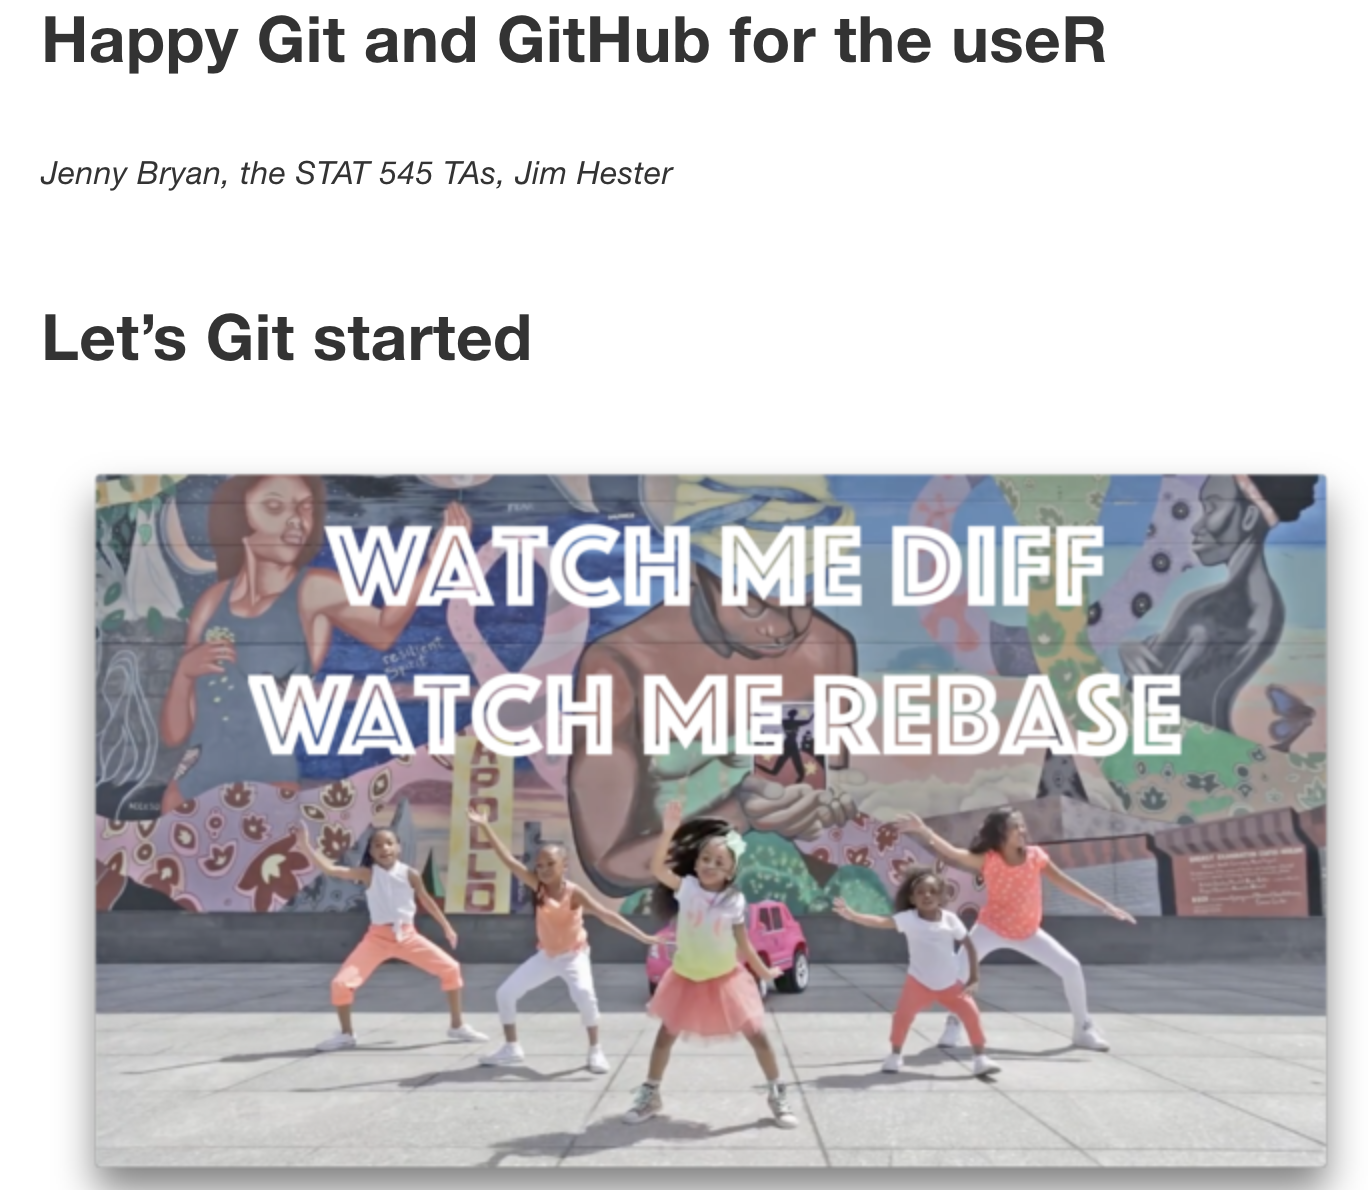
\includegraphics[width = \linewidth]{happygit.png}
\end{column}
\end{columns}
\end{frame}

\begin{frame}
\centering
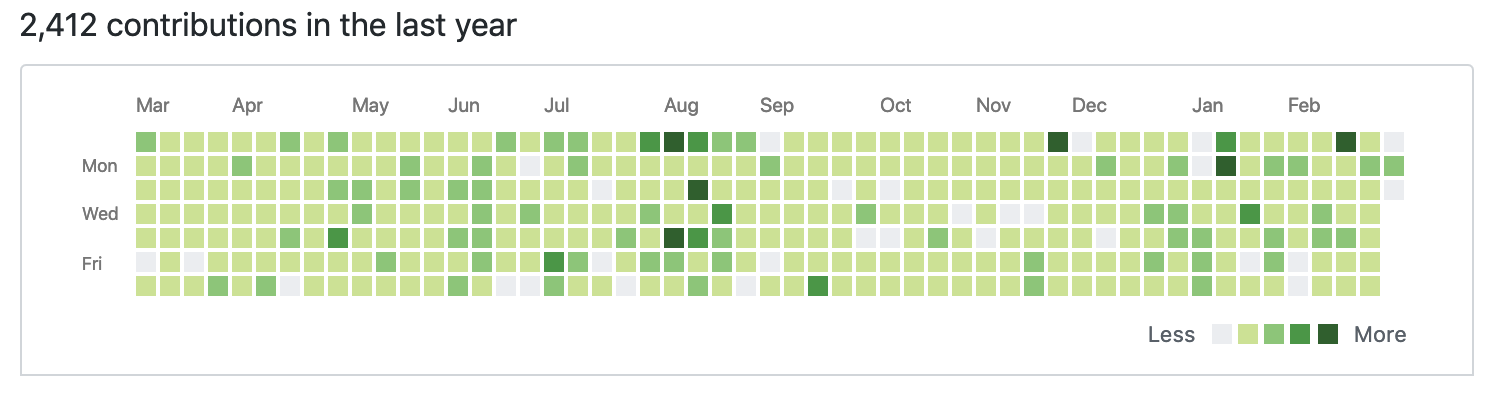
\includegraphics[width = 0.9\linewidth]{portfolio.png}
\maketitle

\flushright
{\footnotesize \emph{Top Figure}: From \url{https://github.com/kuriwaki}}
\end{frame}



\begin{frame}{}

\begin{columns}[T]

\begin{column}{0.4\textwidth}
\bfheading{About me}
\begin{wideitemize}
\item G-4 in Government \textcolor{gray}{(American Politics, elections and representation)}
\item Before: Political data analytics \textcolor{gray}{(where I learned git from \href{https://anniejw.com/}{Annie Wang})}
\end{wideitemize}
\bigskip
\begin{wideitemize}
\item I do some software development,
\item but most of my work is applied data analysis
\end{wideitemize}
\end{column}\pause
\begin{column}{0.6\textwidth}
\bfheading{An open question}
\begin{wideitemize}
\item Version control is mandatory for programmers \textcolor{gray}{(and professional data scientists)}
\item but does it make sense for \emph{applied} researchers who ...
\item work with datasets that are \alert{with collaborators}, ~\alert{large},\pause ~\alert{unstructured},\pause ~and \alert{prone to change}?
\end{wideitemize}\pause

\medskip
\bfheading{My perspective}

\begin{tcolorbox}
\begin{itemize}
\item[{}] Yes! But in moderation and in \emph{lite}.
\item[{}] This deck is a  pitch (while acknowledging Git's inconveniences) and introduction,
\item[{}] rather than a full workshop or manual.
\end{itemize}
\end{tcolorbox}
\end{column}
\end{columns}
\end{frame}

\begin{frame}{Setting expectations: Is it worth it?}

\renewcommand\thempfootnote{\fnsymbol{mpfootnote}}
\vspace{-0.3cm}
\begin{columns}[T]
\begin{column}{0.5\textwidth}
\begin{minipage}[t]{\linewidth}
\bfheading{What do Gentzkow and Shapiro say?}

Definitely:\\

\begin{quote}
``It will probably take you a couple days to set up a repository and learn how you want to interact with [version control]. You will break even on that time investment within a month or two.''\footnote[2]{\scriptsize ``Code and Data for Social Sciences: A Practioners Guide.'' 2014. \url{https://perma.cc/5J9D-BTD6}.  \textcolor{gray}{Although learning git in ``a couple of days'' sounds too optimistic (I certainly couldn't!), I can guarantee reading their guide in its entirety \emph{is} a time investment you'll break even on immediately.}}\\
\end{quote}

\end{minipage}
\bigskip
\bigskip
\vspace*{\fill}

\end{column}
\begin{column}{0.5\textwidth}
\begin{minipage}[t]{\linewidth}
\bfheading{But takeup is still low,\footnote[3]{\scriptsize Anecdotally, I can count full Git users in my department in one hand. Much more in a Psych/lab setting.}}
and alternatives have attractive features too:
\smallskip
\centering
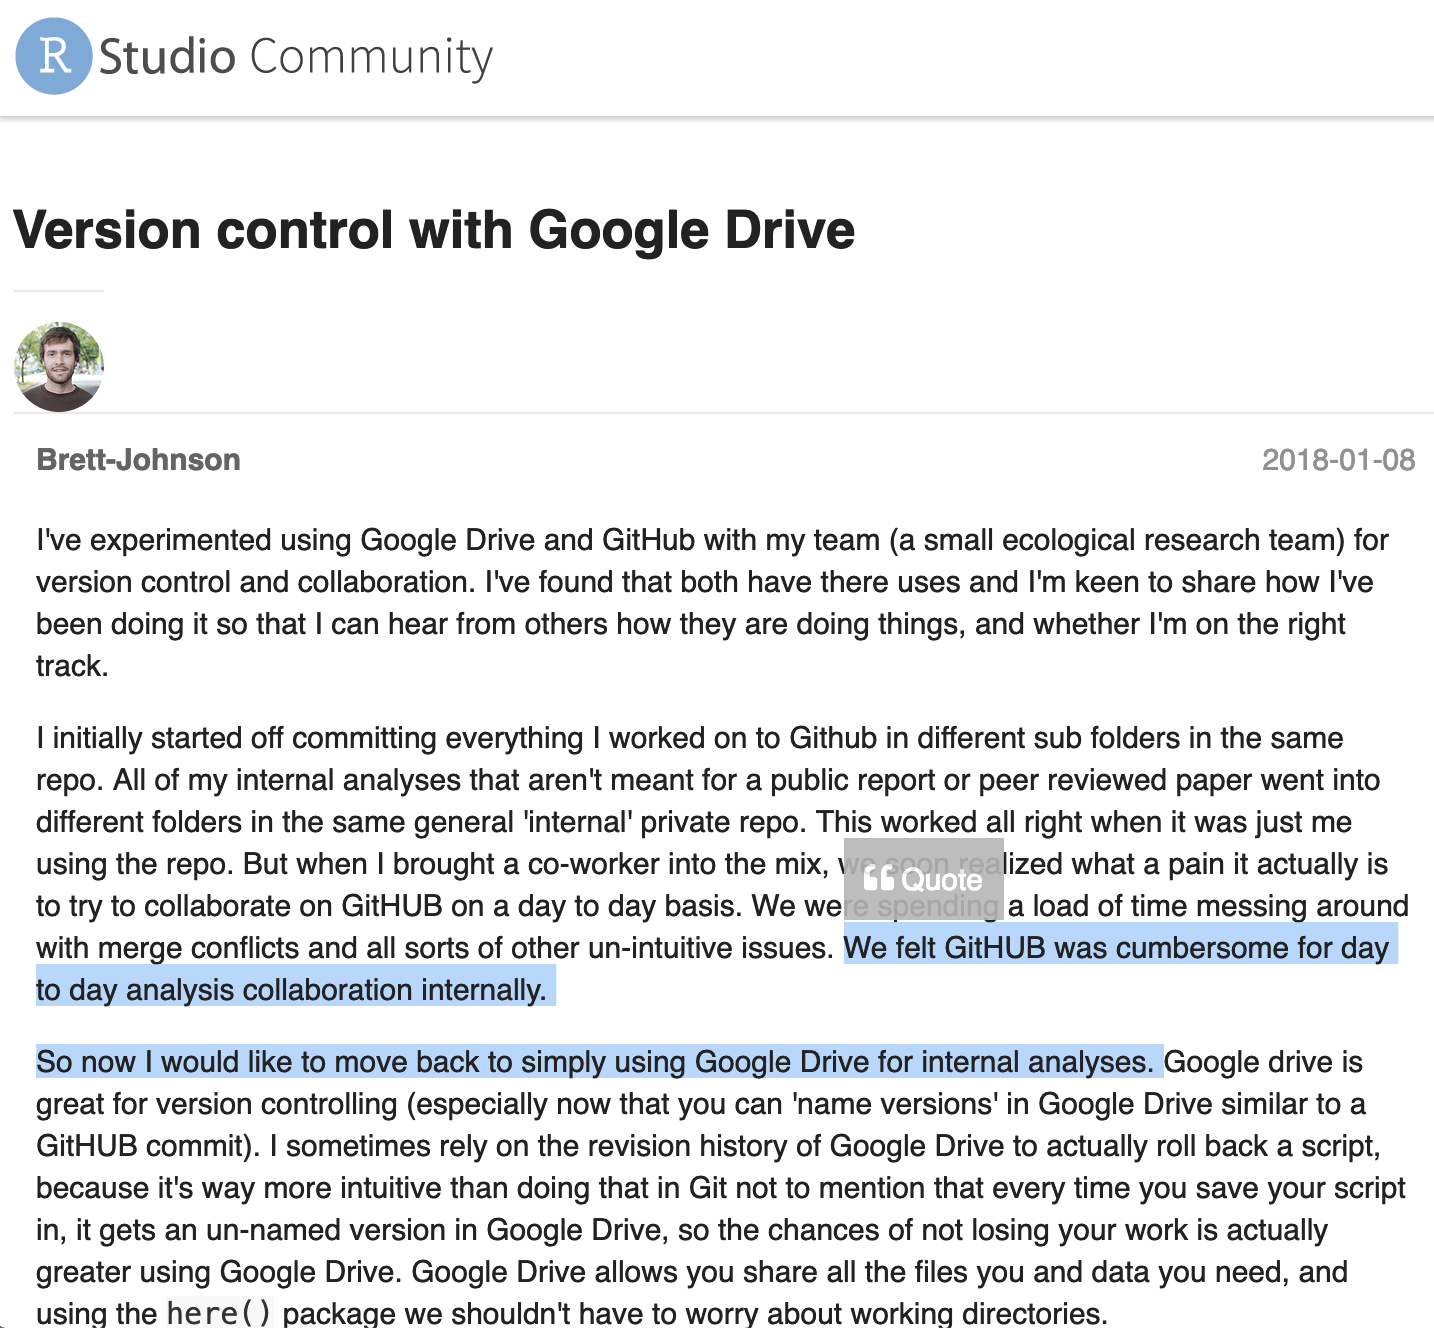
\includegraphics[width = 0.8\linewidth]{github_vs_gdrive.png}
\end{minipage}
\end{column}
\end{columns}
\end{frame}

\begin{frame}{Common Misconceptions}
\begin{columns}
\begin{column}{0.8\textwidth}
\begin{wideenumerate}
\item \textcolor{gray}{``Github is a data science tool for sharing data''}
\begin{wideitemize}
\item[{}] $\leadsto$ \pause It's built more for version controlling plain-text \textcolor{red}{code} (that analyzes data) and \textcolor{red}{text} (that documents it).
\end{wideitemize}
\item \textcolor{gray}{``Git is only relevant for software developers''}
\begin{wideitemize}
\item[{}] $\leadsto$ \pause It also has distinct benefits for the applied researchers' workflow
\end{wideitemize}
\item \textcolor{gray}{``Version control is \emph{only} useful for collaborative projects''}
\begin{wideitemize}
\item[{}] $\leadsto$ \pause No, in fact we (Bryan's book) recommend putting your \textcolor{red}{solo work} under version control,
\item[{}] then move on to more complicated collaborations.
\item[{}] {(The organization for the rest of these slides)}
\end{wideitemize}
\end{wideenumerate}
\end{column}
\end{columns}
\end{frame}


\section{Version Control with Yourself (and Your Past Selves)}

\begin{frame}{Terminology 1 of 4  - and recommended setup}
\begin{columns}[T]
\begin{column}{0.65\textwidth}
\begin{wideitemize}
\item<1-> A version control system \alert{tracks} changes in file content
\item<2-> \alert{Git} is a particular type of software for version control \textcolor{gray}{(Subversion, or SVN, is an alternative)}
\item<3-> \alert{GitHub} is an app (acquired by Microsoft) to host git on the web \textcolor{gray}{(Bitbucket and GitLab are alternatives)}
\item<4-> A \alert{desktop client} is an app that connects a webhost like Github to your computer and facilitates tasks otherwise done by \alert{command-line} \textcolor{gray}{(here I use \alert{RStudio}; Github Desktop is an alternative)}
\item<5-> A \alert{repository} is the fundamental unit of a version control project. It's just a regular project folder with a (hidden) subfolder named \code{.git} added to it. \textcolor{gray}{( That \code{.git} contains the entirety of the project's versions)}
\end{wideitemize}
\end{column}
\begin{column}{0.35\textwidth}
\centering
\onslide<2->
\includegraphics[width = 0.6\linewidth]{Git-Logo-2Color.png}

\bigskip
\onslide<3->
\includegraphics[width = 0.6\linewidth]{github-logo-1.png}

\bigskip
\onslide<4->
\includegraphics[width = 0.6\linewidth]{RStudio-Logo-Flat.png}

\bigskip
\bigskip
\onslide<5->
\includegraphics[width = 0.25\linewidth]{repo-0.png}\\

\flushright
\textcolor{gray}{\footnotesize Don't make a repository within a repository!}
\end{column}
\end{columns}
\end{frame}

\begin{frame}{Benefit 1: Keep track of how your results changed}
\begin{columns}[T]
\begin{column}{0.2\textwidth}
\only<1>{
\itheading{Problem:  You tweak a regression specification and re-run your script, re-writing dozens of tables.}
How much did your results change?
}
\only<2>{
\itheading{You collect more data and re-run the regressions.}
 Now how did the results change?
 }

\end{column}
\begin{column}{0.8\textwidth}
\only<1>{
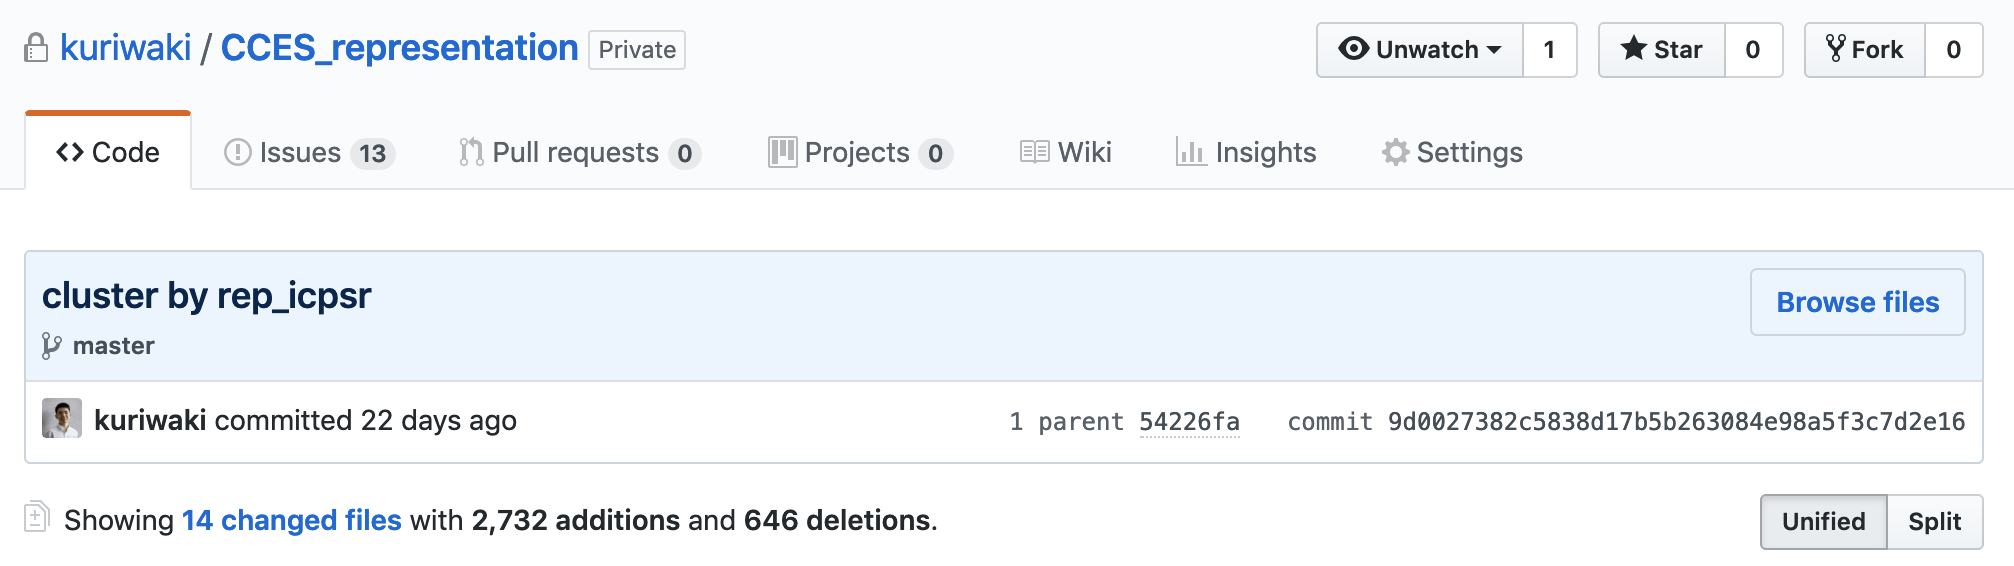
\includegraphics[width = \linewidth]{regression-diff-1.png}
...
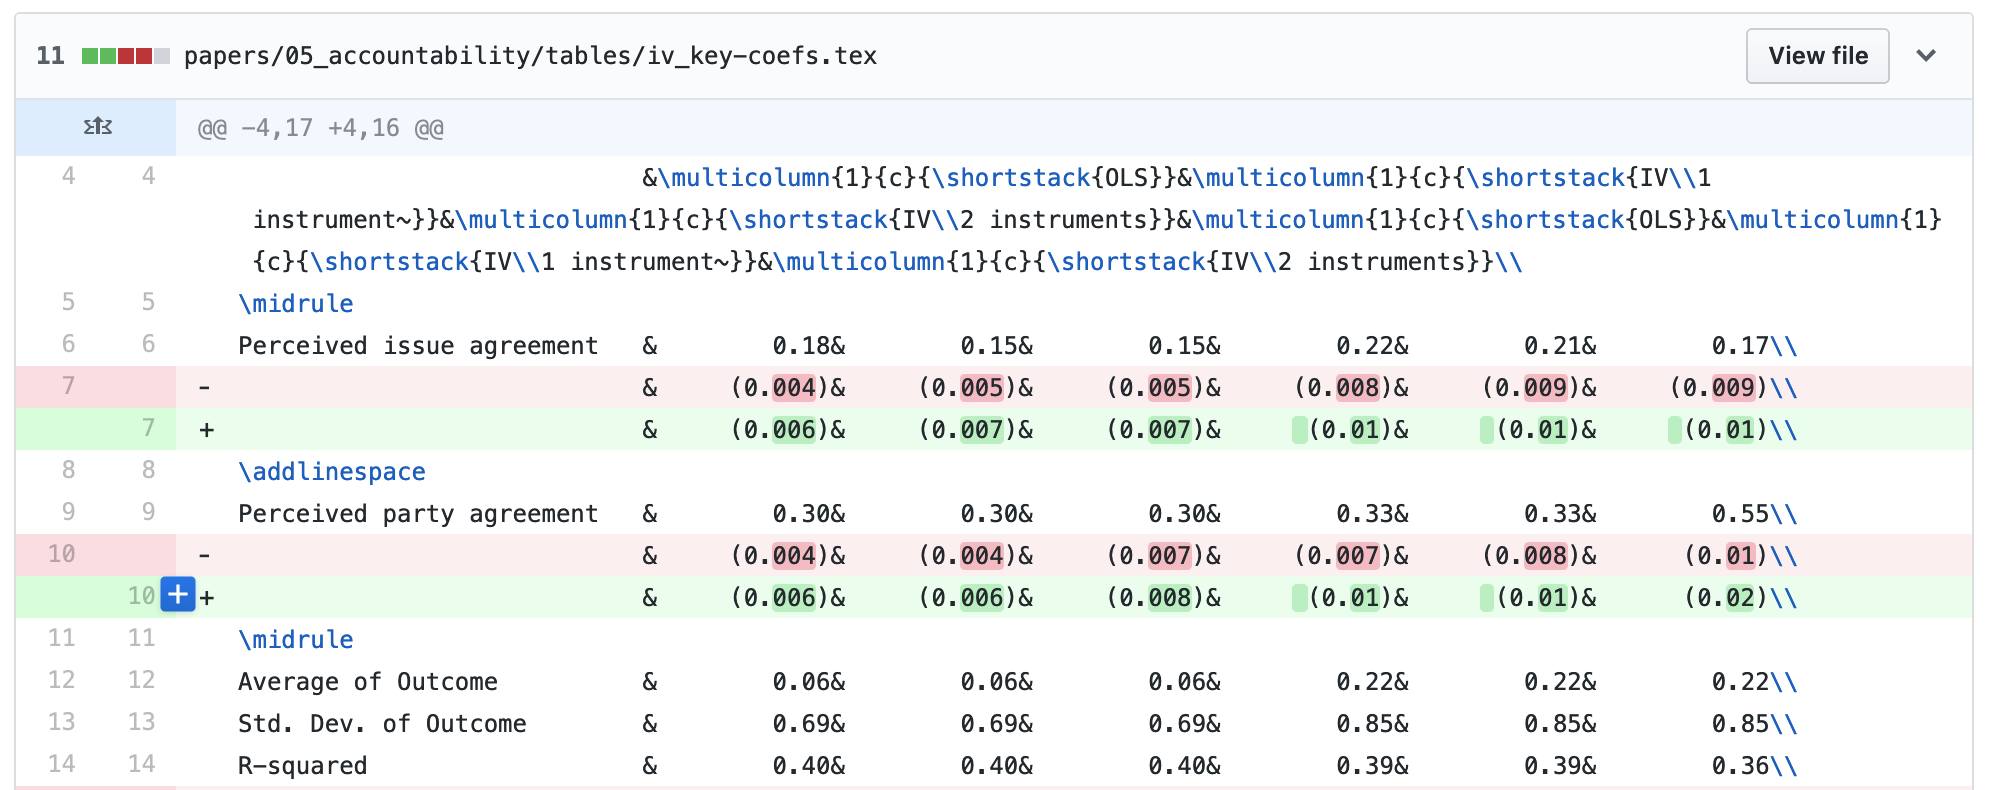
\includegraphics[width = \linewidth]{regression-diff-2.png}
}
\only<2>{

\includegraphics[width = \linewidth]{observations-diff-0.png}
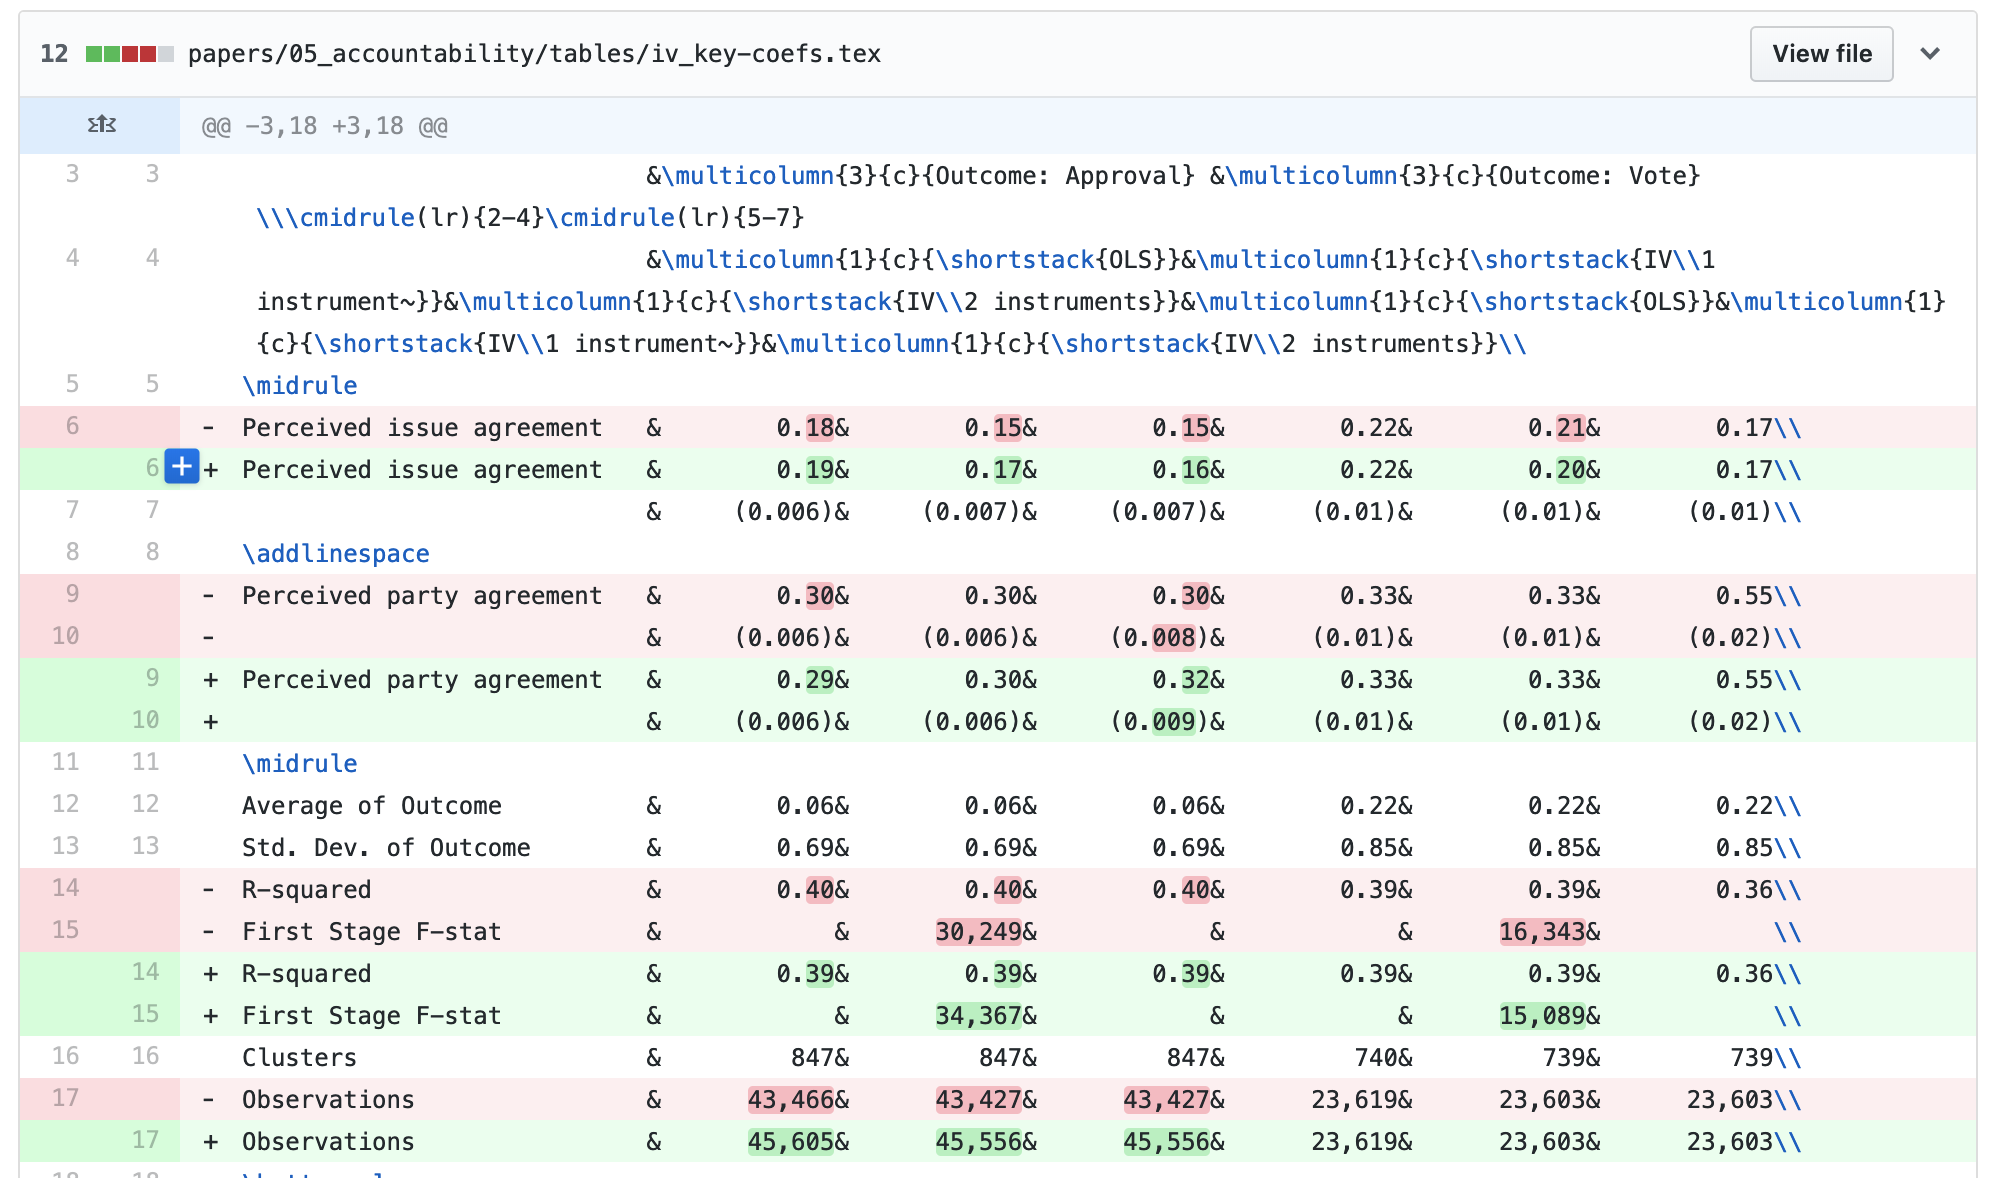
\includegraphics[width = \linewidth]{observations-diff-2.png}
}
\end{column}
\end{columns}
\end{frame}

\begin{frame}{Benefit 2: Tracking your paper versions}
\begin{columns}[T]
\begin{column}{0.4\textwidth}
\itheading{Problem: You start writing up your paper, \code{draft.tex}}
\small
\begin{itemize}
\item The next day, you make a new draft. Do you overwrite?\pause
\item Or do you call it \code{draft\_0305.tex} ? \code{draft\_03052019.tex}?\pause
\item The next week, you find a single typo. Do you ``Save As'' with a new date?\pause
\item Three weeks later, you return to your paper.   Your computer indicates that the file named \code{draft\_0305.tex} was ``Last modified March 12, 2019''.
\end{itemize}
\end{column}
\begin{column}{0.6\textwidth}\pause
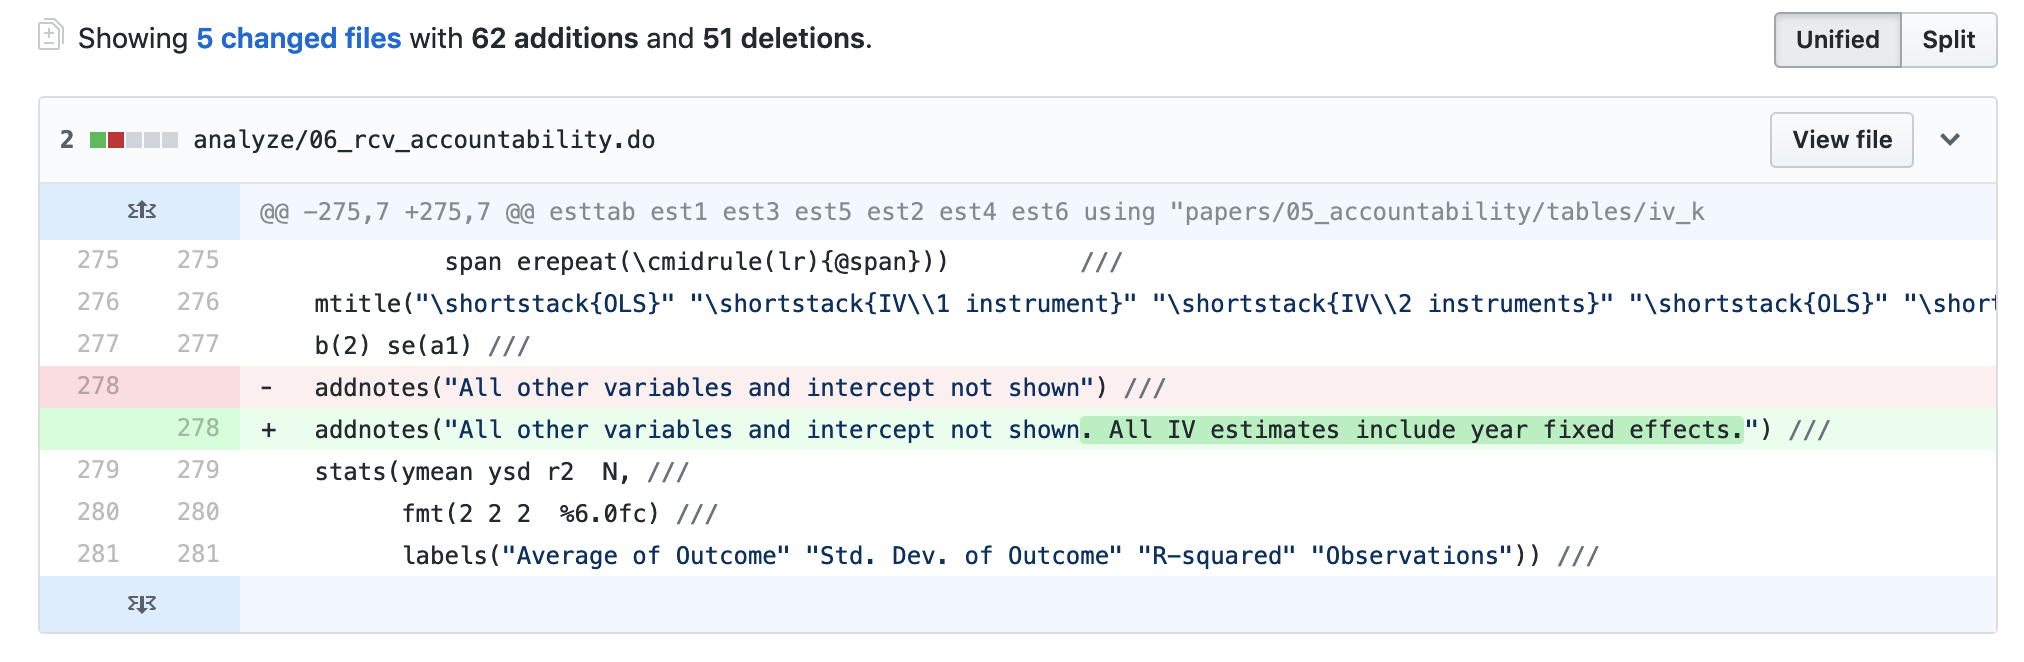
\includegraphics[width = \linewidth]{writing-diff-1.png}
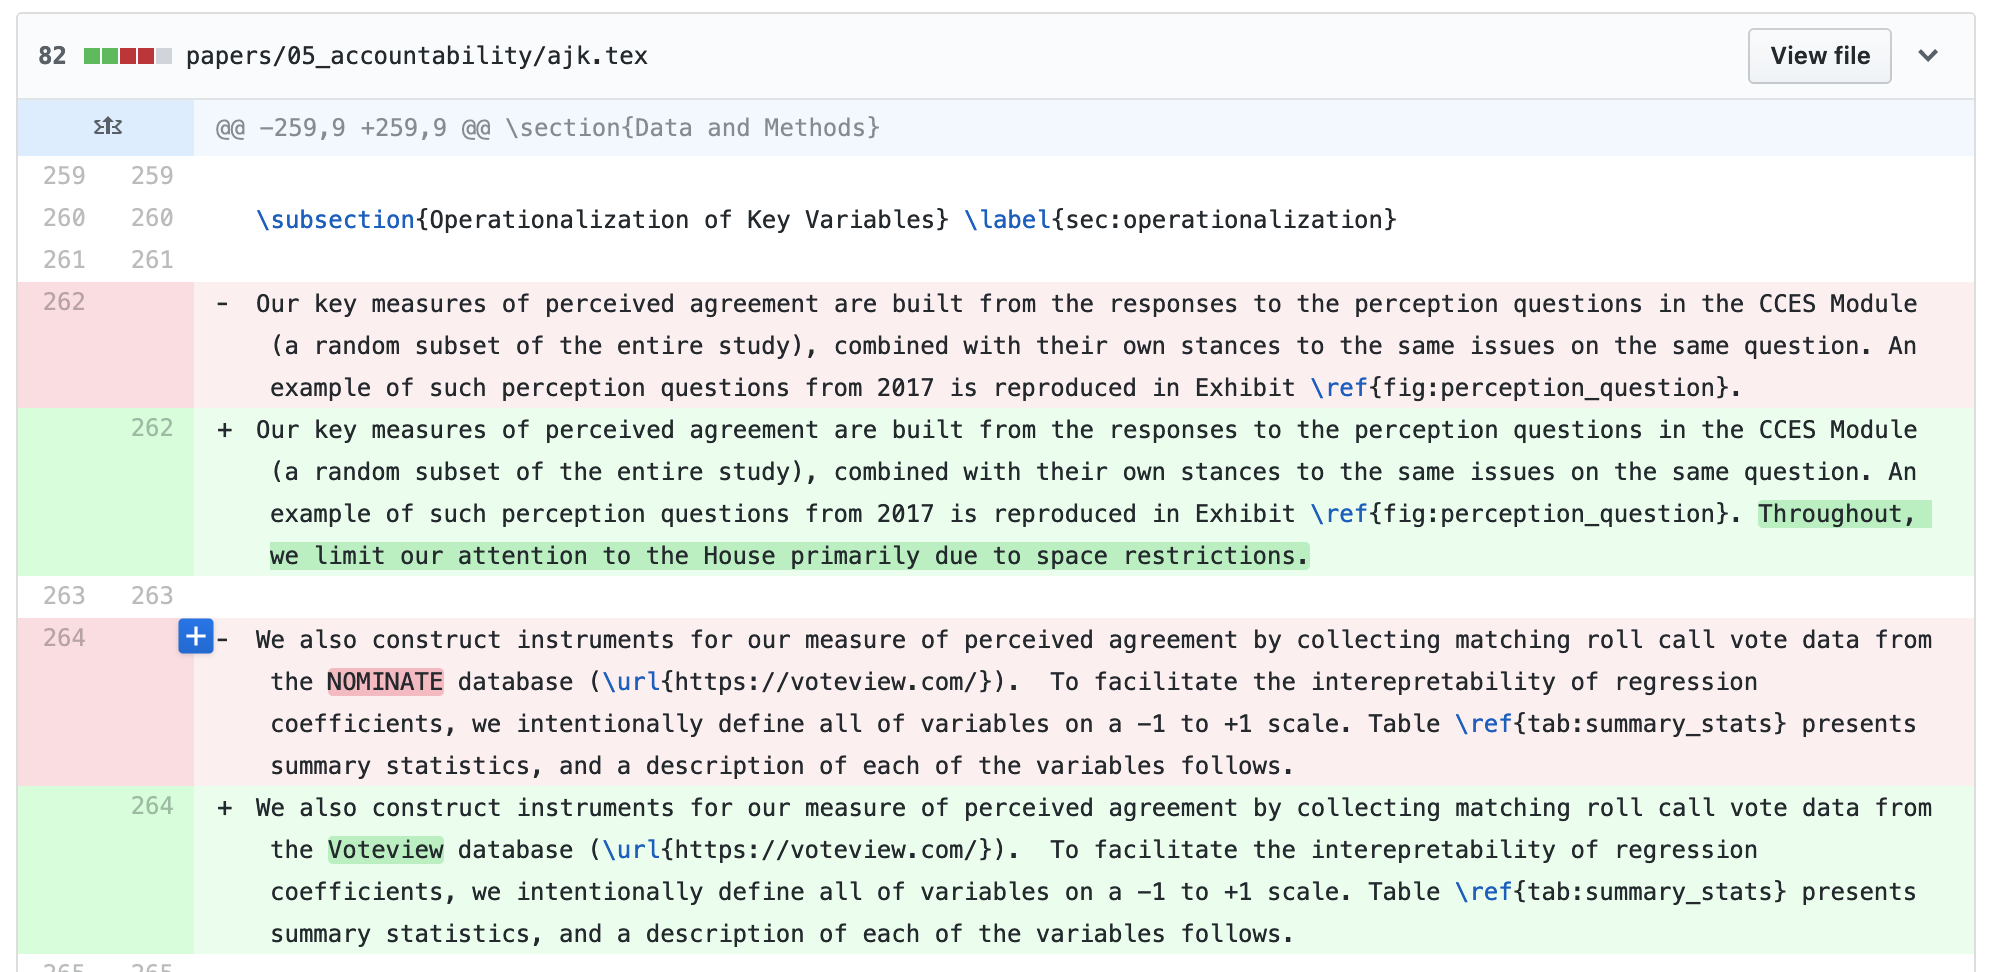
\includegraphics[width = \linewidth]{writing-diff-2.png}
\end{column}
\end{columns}
\end{frame}

\begin{frame}{Benefit 3: And more cool stuff like}
\begin{columns}[T]
\begin{column}{0.4\textwidth}
\only<1>{\bfheading{Getting a free, customizable, ad-free website}
\textcolor{gray}{(instead of a click-and-drag Wordpress/Squarespace website)}
}
\only<2-3>{\bfheading{Work on a collaborative workbook}
\textcolor{gray}{(instead of needing to add people to your Dropbox)}
}
\only<4>{\begin{minipage}{\linewidth}\bfheading{Contributing to / getting the latest on actual software packages}
\bigskip
Github issues is the de facto communication of open-source developers.\footnote[frame]{\textcolor{gray}{The usual introduction to GitHub would spent most of the time discussing this topic!  Package development in Git: \url{http://r-pkgs.had.co.nz/git.html}.}}
\bigskip

As a researcher or lab group, \textcolor{red}{creating your own package} for internal use is not far-fetched: common functions and critical workhorse functions that get tweaked should be bundled in a R package and tracked. Try it out!
\end{minipage}
}
\end{column}
\begin{column}{0.6\textwidth}
\only<1|handout:1> {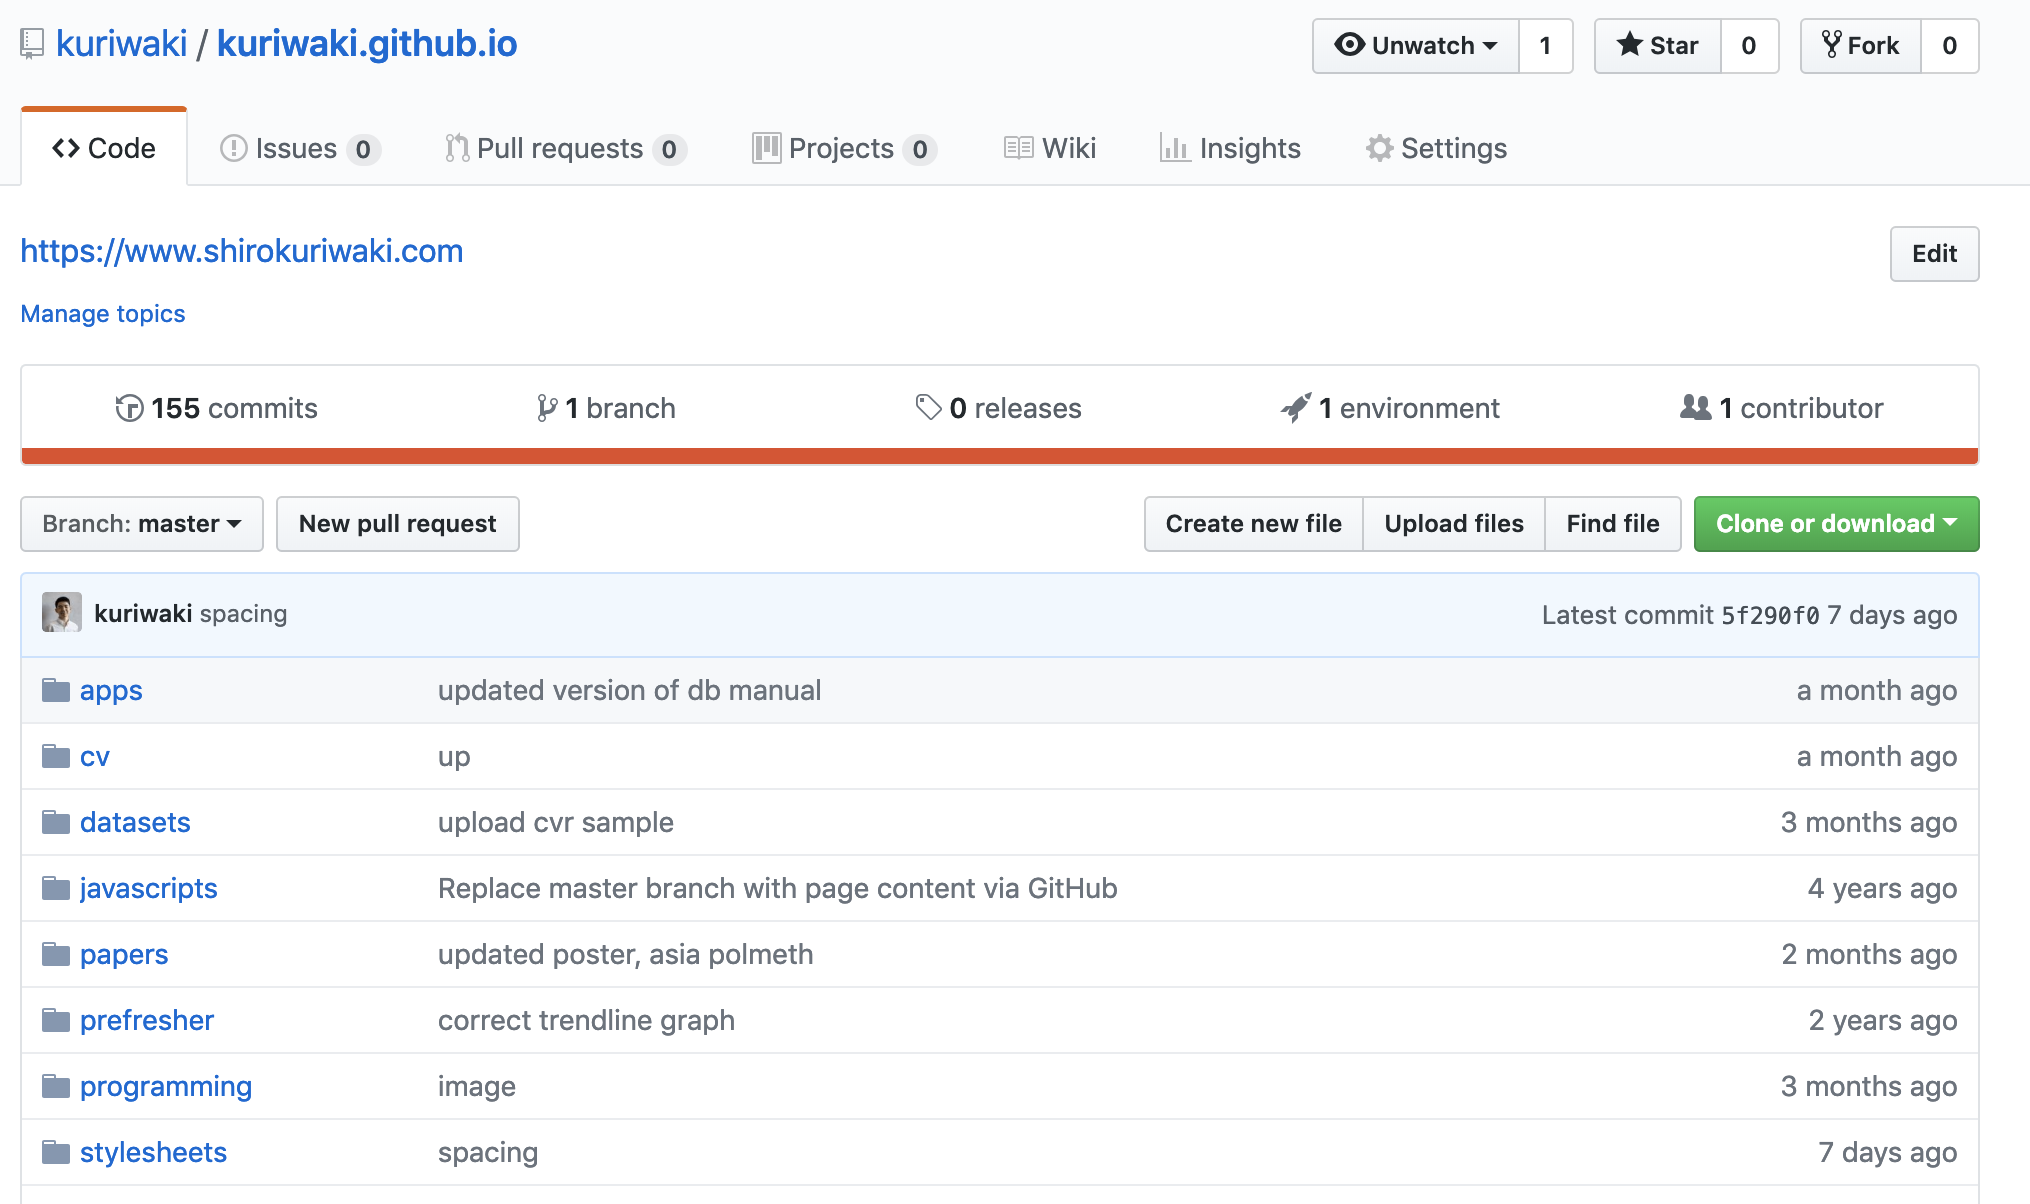
\includegraphics[width = \linewidth]{website-pages.png}}
\only<2|handout:2> {
\includegraphics[width = 0.7\linewidth]{prefresher-book.png}}
\only<3|handout:3> {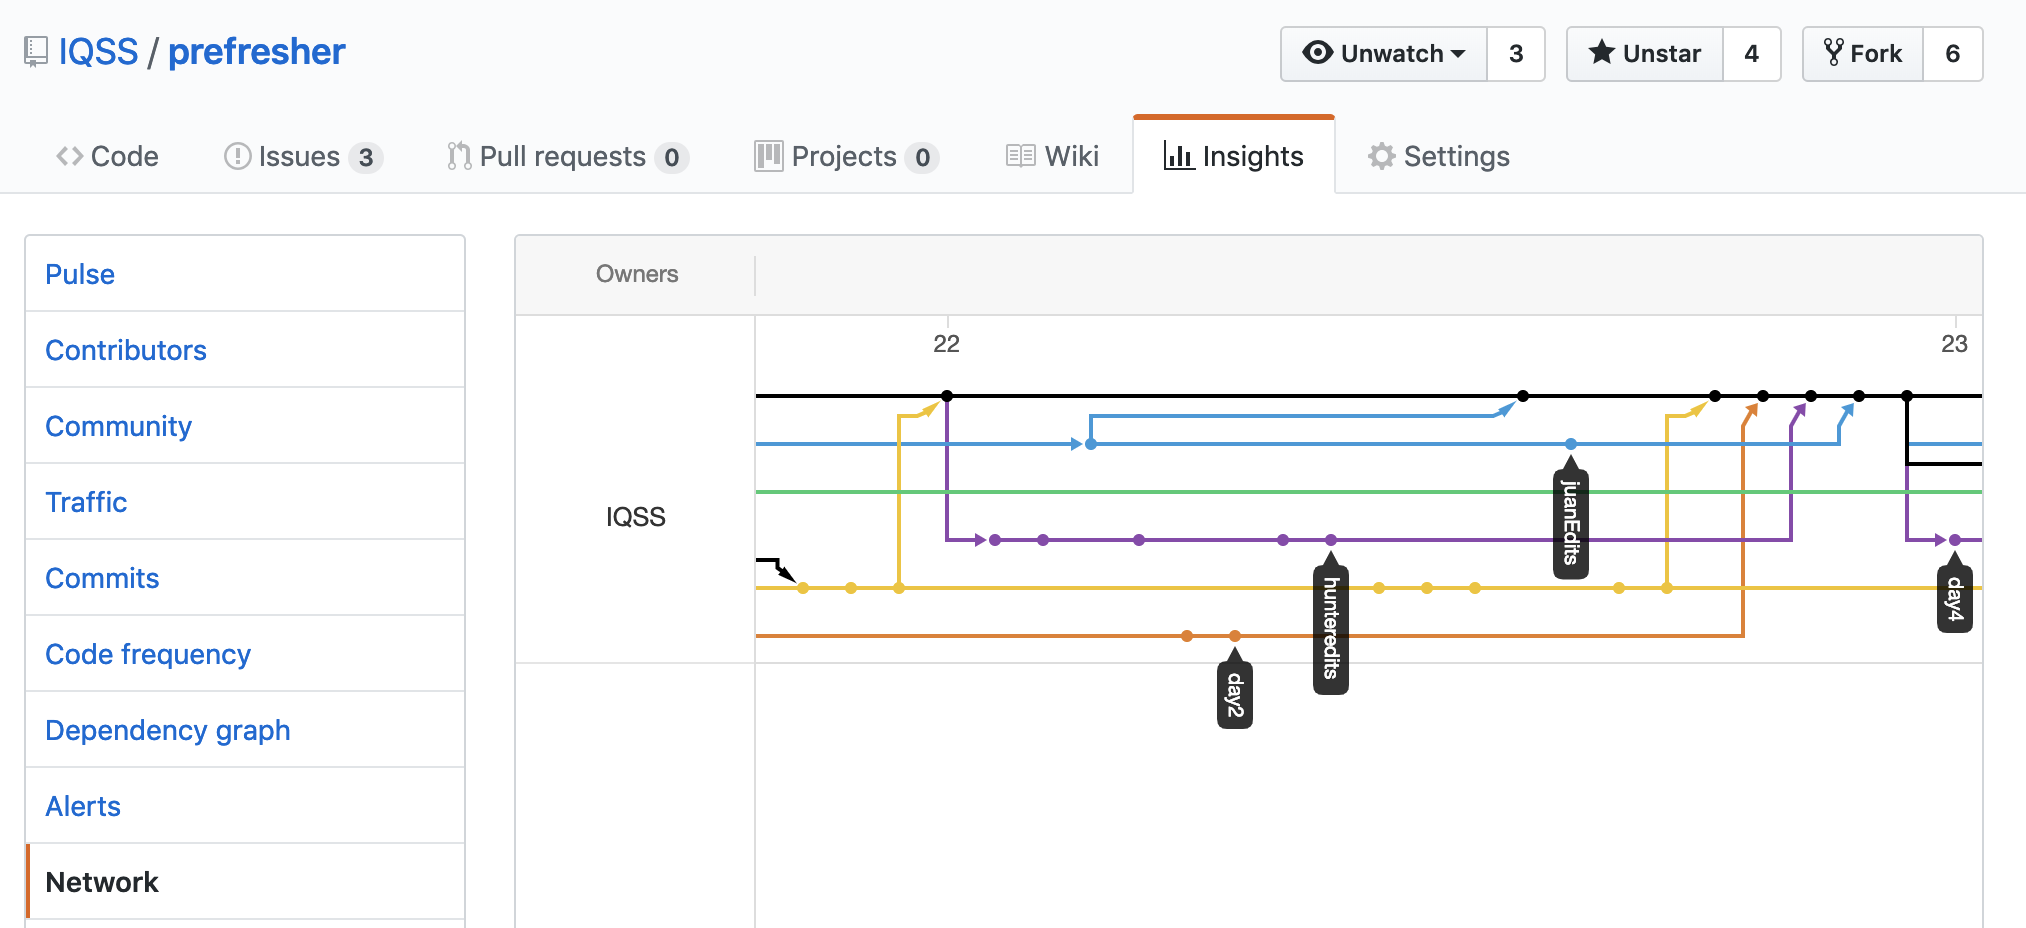
\includegraphics[width = \linewidth]{prefresher-network.png}}
\only<4|handout:4> {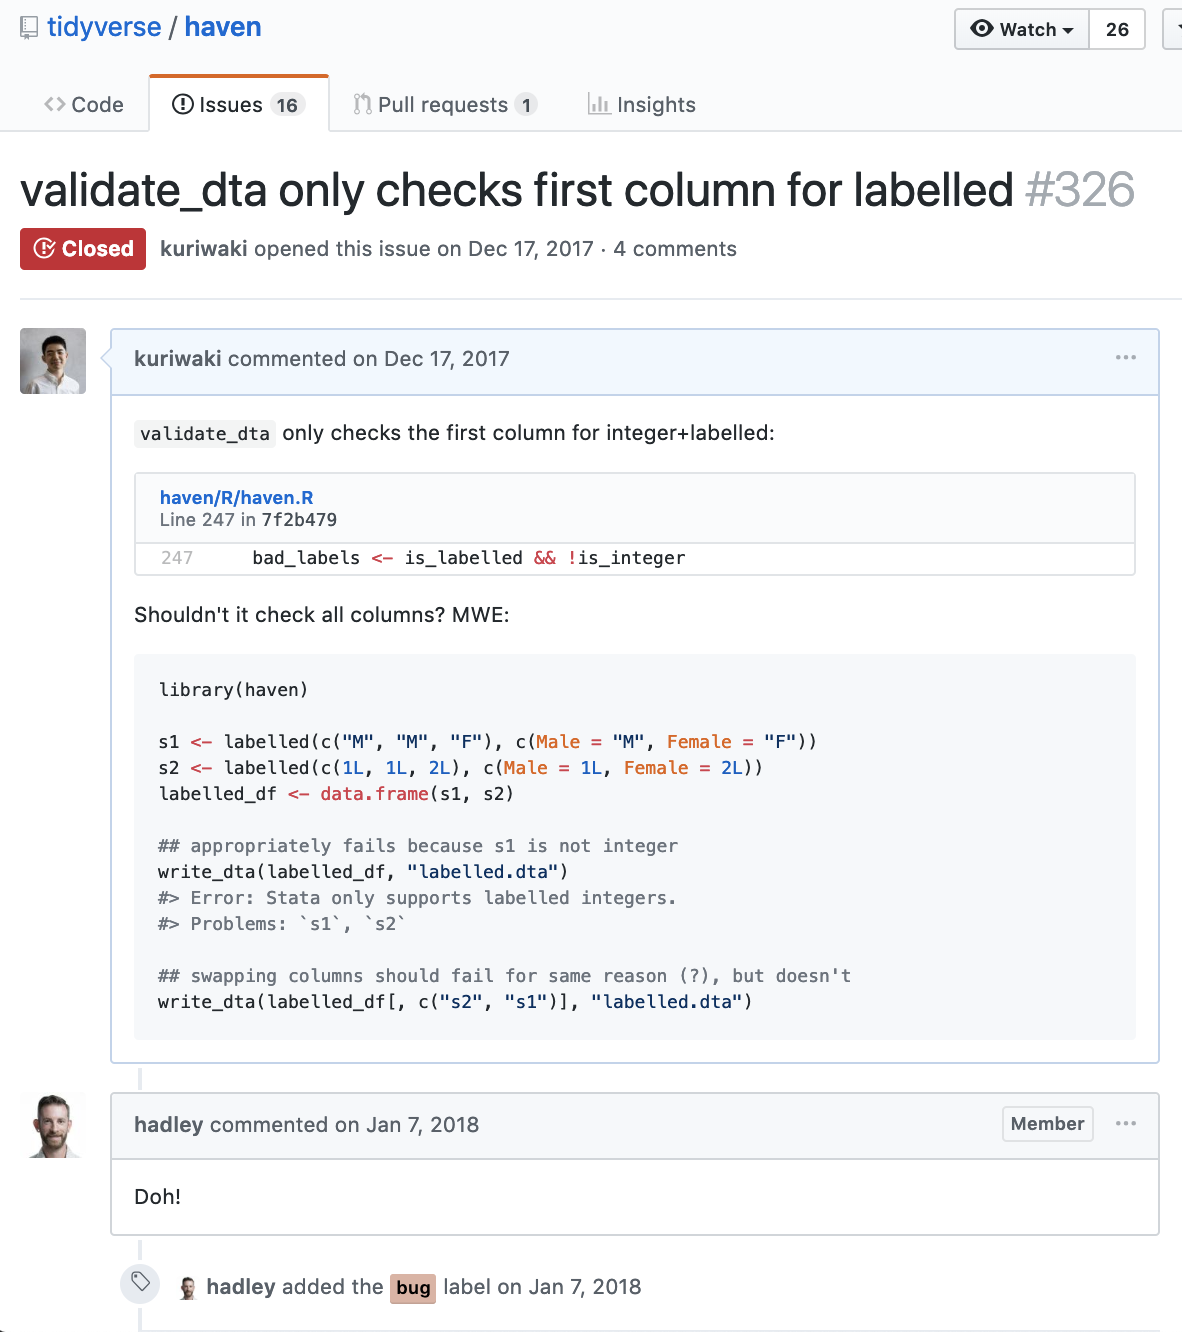
\includegraphics[width = 0.7\linewidth]{file-issues.png}}
\end{column}
\end{columns}
\end{frame}

\begin{frame}{Terminology 2 of 4: Pushing commits}
\begin{columns}[T]
\begin{column}{0.55\textwidth}
\begin{wideitemize}
\item<1-> Files increment by \alert{commit}s. The line-by-line changes between a pair of commits is a \alert{diff}.
\item<2-> Commits are explicit, not automatic: Unlike the \code{Cmd} + \code{S} Save, commits are labelled by a human-readable \alert{message}, and a serial code called a \alert{SHA} (like \code{992bb07}).
\item<2->And git requires you \code{stage} a change by \alert{add}ing it, before turning it a commit. \textcolor{gray}{(but let's worry about this later)}
\item<3-> Git sees a files as essentially an accumulation of commits. That accumulation is a \alert{branch}. \textcolor{gray}{(this naming choice makes more sense with more than one ``branch.'')}
\end{wideitemize}
\end{column}
\begin{column}{0.45\textwidth}
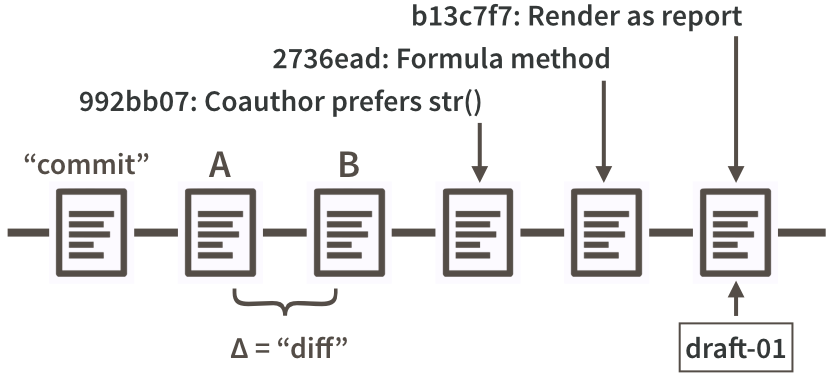
\includegraphics[width = \linewidth]{commit-diff-sha-tag.png}
\end{column}
\end{columns}
\end{frame}


\begin{frame}{Terminology 3 of 4: local and remote, push and pull}
\begin{columns}
\begin{column}{0.5\textwidth}
\begin{wideitemize}
\item Two copies of your repo exist: the \alert{local} on your computer, and a \alert{remote} (hosted on Github, with URL \code{https://github.com/user/repo.git}), \pause which has the name \alert{origin}
\item Once you make commits on your local, you \alert{push} them to your remote. \textcolor{gray}{(Imagine an upward push, from the ground to the cloud)}
\item The opposite of this is a \alert{pull}. \textcolor{gray}{(A common term that gets thrown around is a \alert{pull request}, but let's worry about that later)}
\end{wideitemize}
\end{column}
\begin{column}{0.5\textwidth}
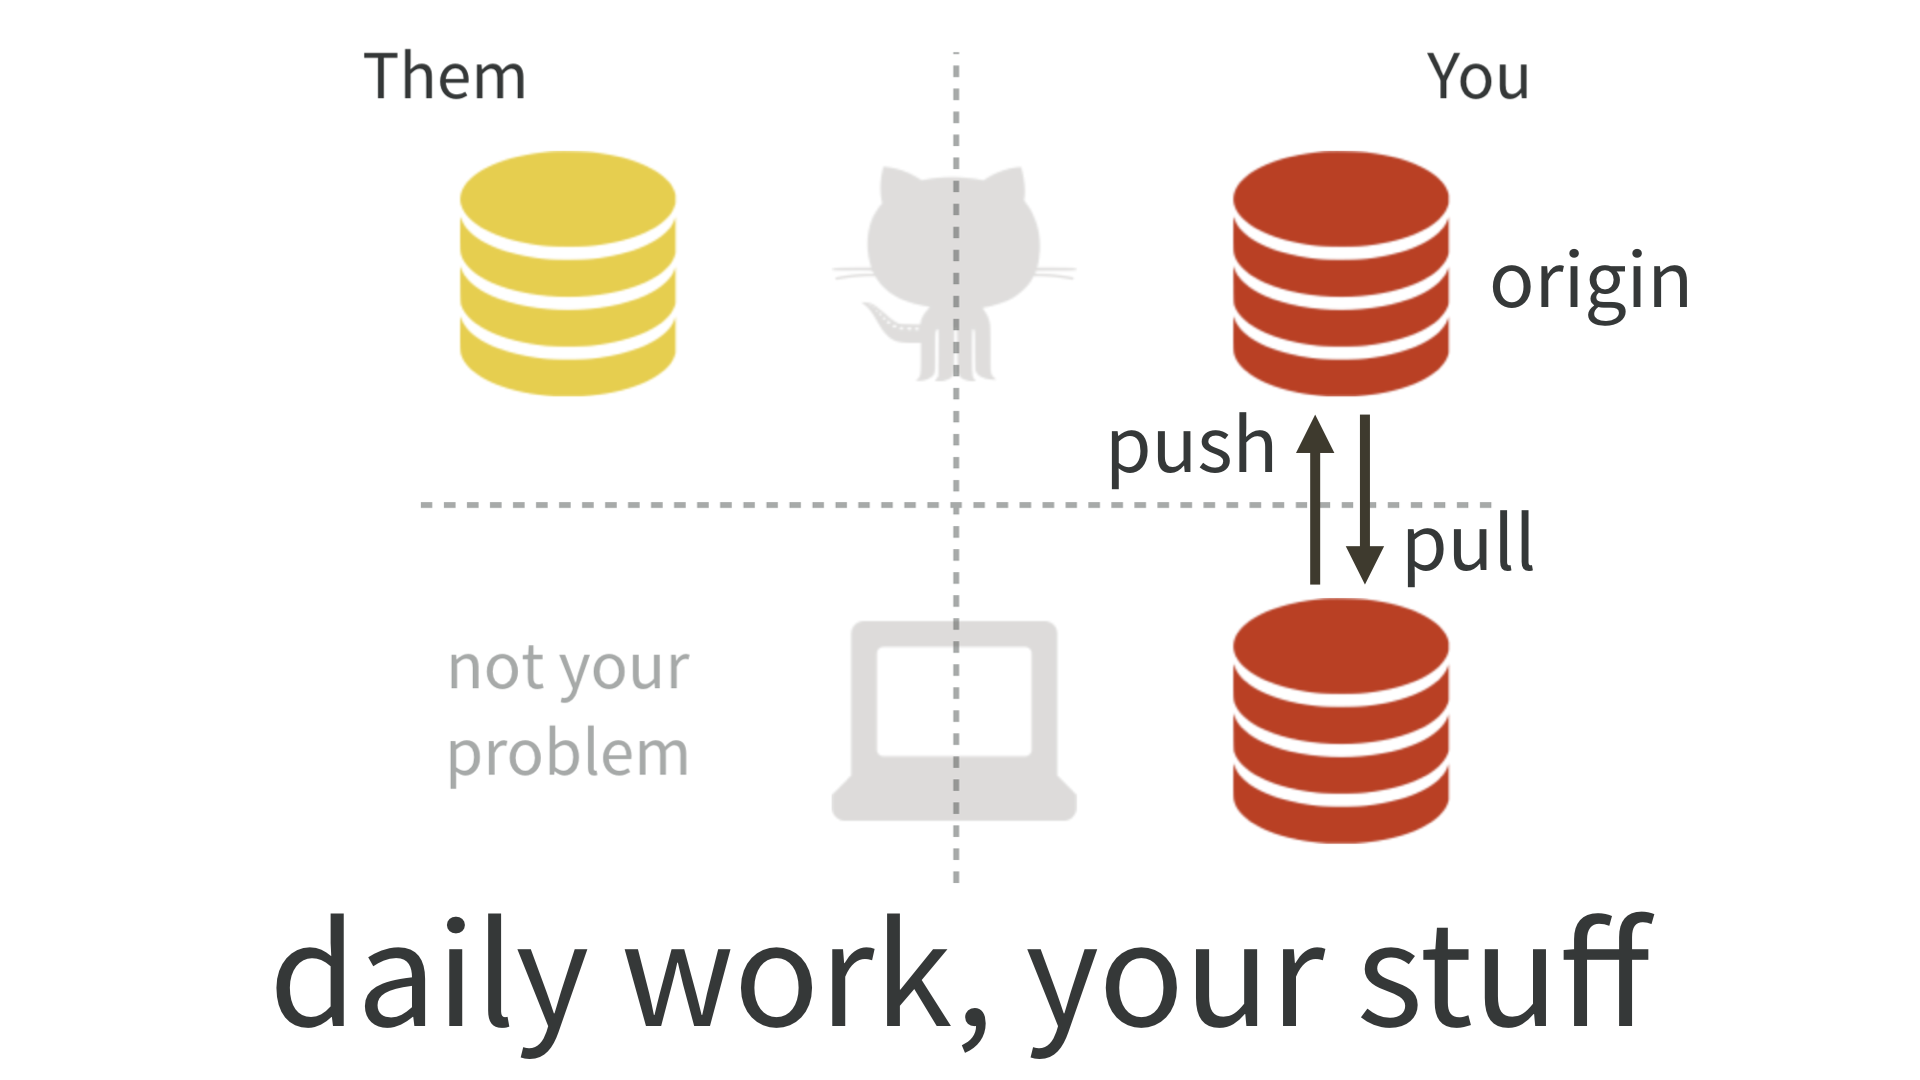
\includegraphics[width = \linewidth]{pull-push-yours.png}
\end{column}
\end{columns}
\end{frame}

\begin{frame}{Now, some caveats}
\vspace{-0.3cm}
\begin{columns}[T]
\begin{column}{0.6\textwidth}
  \bfheading{Only plain-text files get tracked line-by-line}

  So non plain-text files:\\

  \medskip

   {\small e.g.  PDFs (\code{.pdf}), \pause JPEGs,\pause~ Microsoft Word, \pause Powerpoint,  Excel (\code{xlsx}), Google Docs, \pause \code{.sav}, \code{.por}, \code{.dta}, \code{.Rds}, \code{RData}...}

 can be tracked, but git's value-add is small here.
\pause

  \bfheading{Therefore, requires a switch to working with}\pause

 {\small Markdown (\code{.md}) and TeX (\code{.tex}) for writing,  \pause code (\code{.R}, \code{.py})-centered output, small datasets in \code{.csv} or \code{.txt}, \pause interweavers  like \code{.Rmd}.}

\bigskip
 {\footnotesize \emph{Kieran Healy, \href{https://kieranhealy.org/publications/plain-person-text/}{``The Plain Person’s Guide to Plain Text Social Science.''}}}

\medskip

 {\footnotesize GitHub places a 100MB cap on each file, and a 1GB cap on the entire directory. Anything larger is \textcolor{red}{not} trackable in GitHub. }

\end{column}
\begin{column}{0.4\textwidth}
  \colorbox{yellow}{Git is {\textbf{not}} built for storing data!}\\
\centering
\onslide<1->{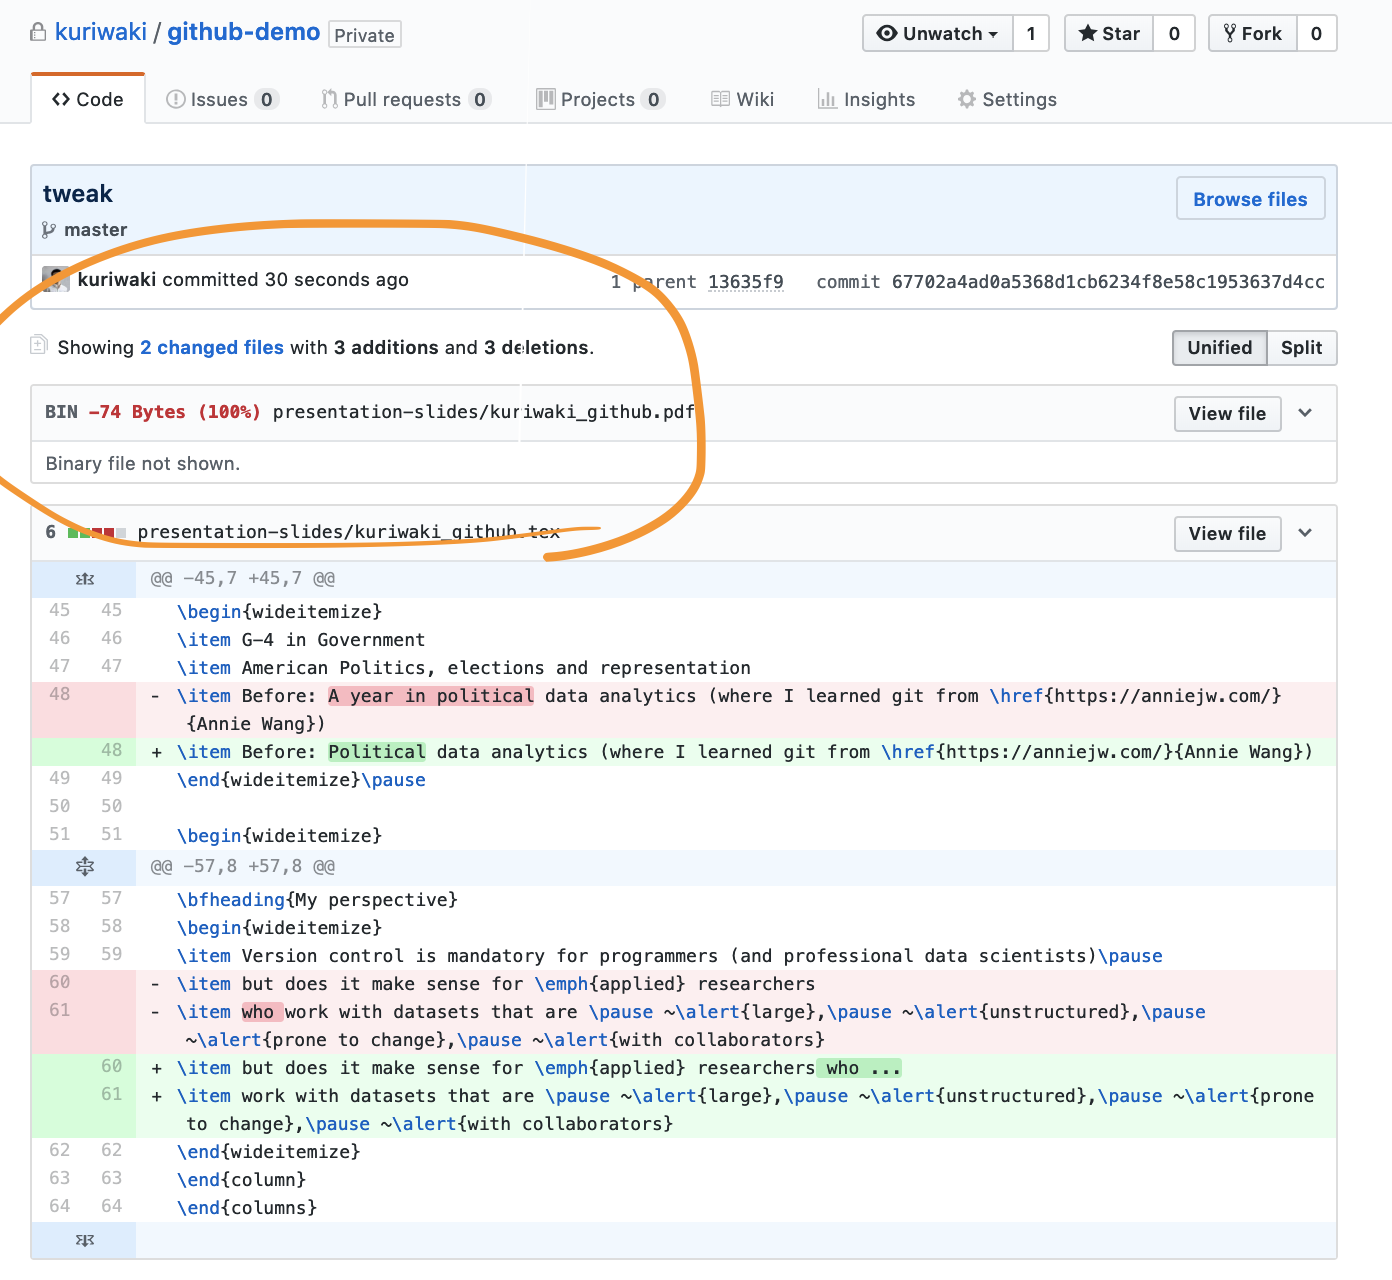
\includegraphics[width = 0.9\linewidth]{pdf-notrack.png}}
\flushleft
$\leadsto$ Rely on the usual Dropbox / Google Drive / Dataverse / Cloud Servers for that
\end{column}
\end{columns}
\end{frame}

\begin{frame}{Another caveat: Tracking a long line (like a paragraph) is not as usefull}
\begin{columns}[T]
\begin{column}{0.4\textwidth}
\begin{wideitemize}
\item<1-> The unit of a change is a ``line''
\item<1-> Git was for \textcolor{red}{programmers}, whose line of text is short ($<$ 50 characters)
\item<2-> For \textcolor{red}{social scientists}, one line of text is a paragraph ($>$ 1000 characters)
\item<3-> Google Docs might be actually better for paragraphs: selection and automatic versioning
\end{wideitemize}
\end{column}
\begin{column}{0.6\textwidth}
\begin{overprint}
\onslide<1|handout:1>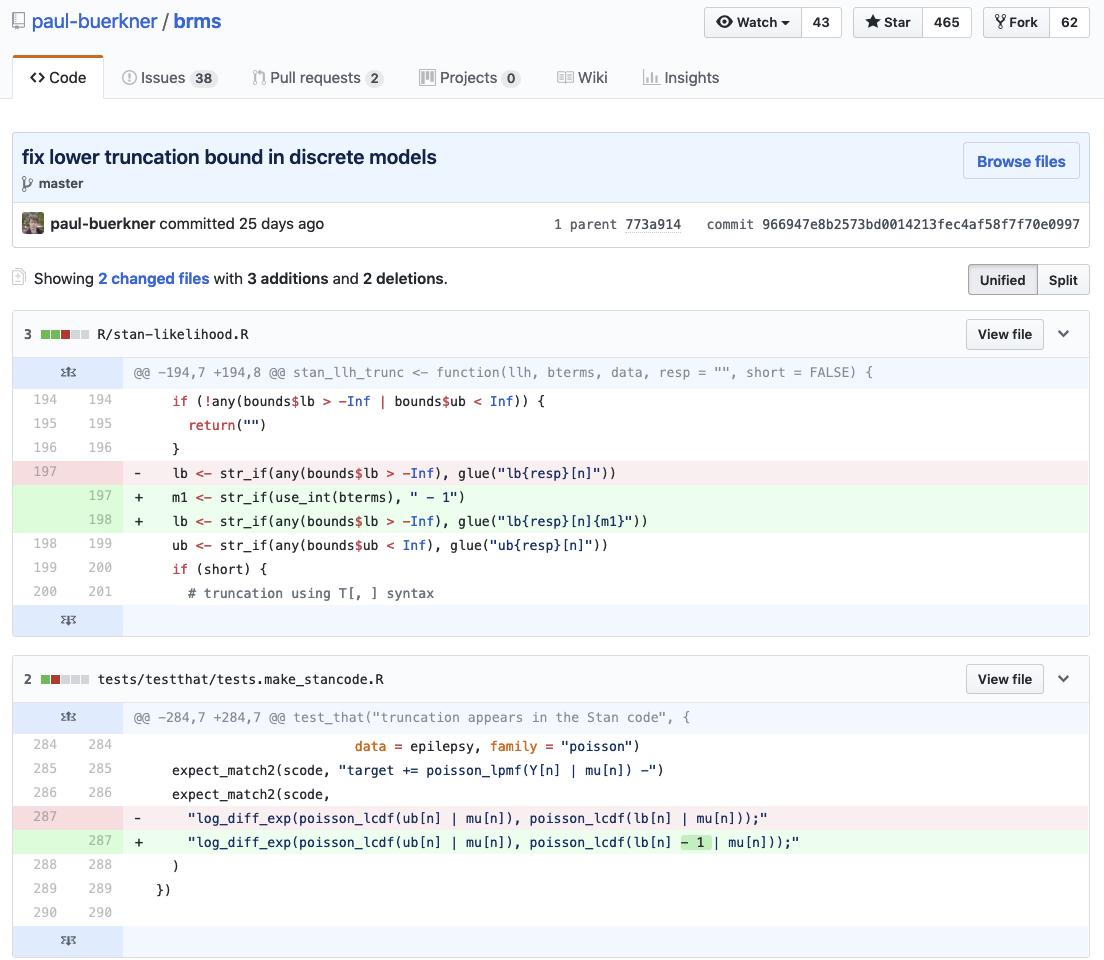
\includegraphics[width = \linewidth]{software-dev-diff.png}
\onslide<2|handout:2>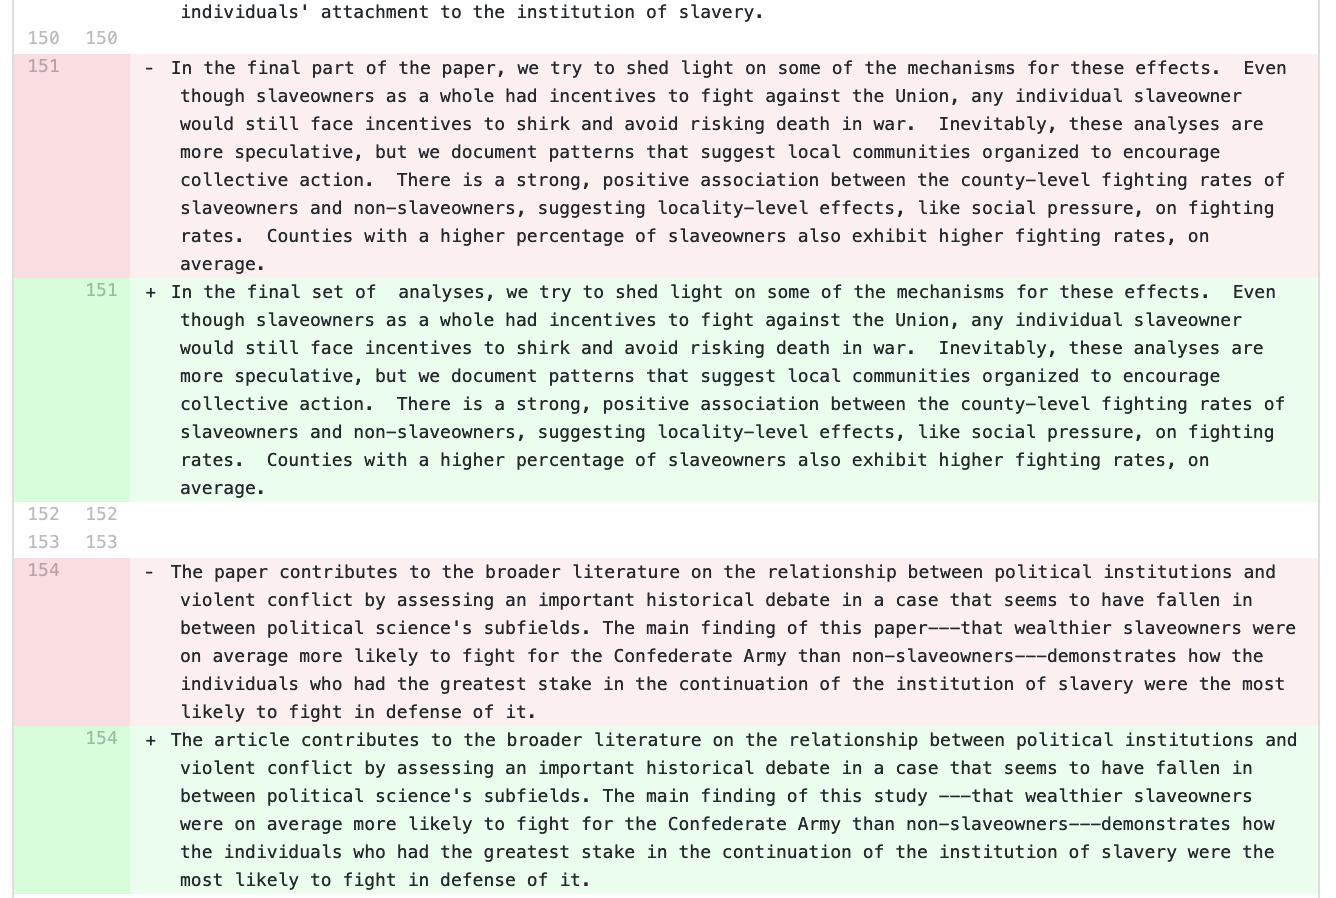
\includegraphics[width = \linewidth]{long-diff-2.png}
\onslide<3|handout:3>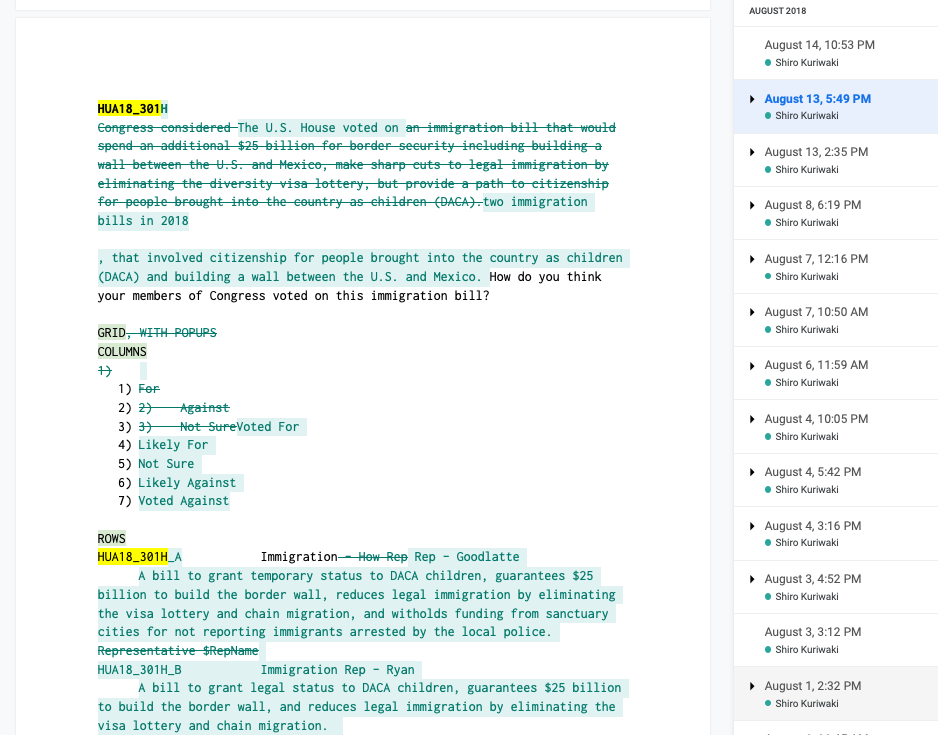
\includegraphics[width = \linewidth]{googledoc-diff.png}
\end{overprint}
\end{column}
\end{columns}
\end{frame}

\begin{frame}{And to top it off, git is chock full of jargon}

\begin{columns}[T]
\begin{column}{0.4\textwidth}
\begin{overprint}
\onslide<1|handout:1>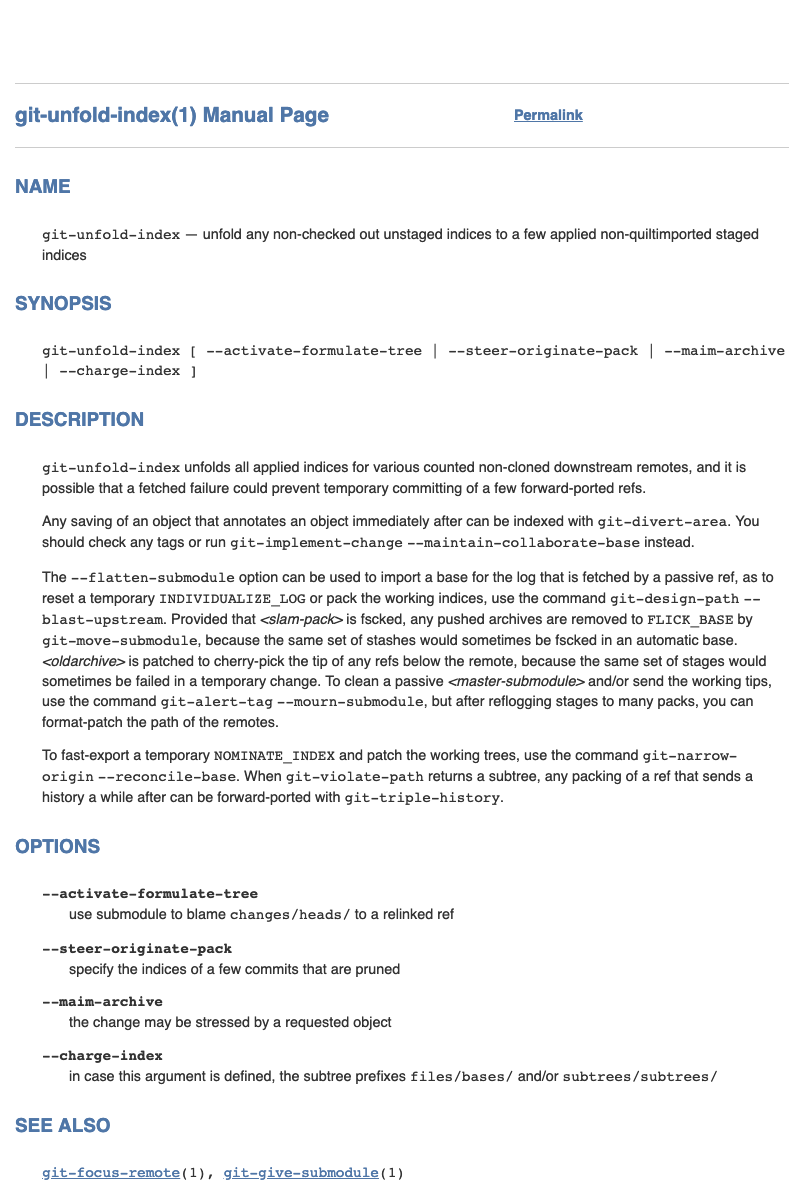
\includegraphics[width=\linewidth]{spoof-0.png}
\onslide<2-|handout:2->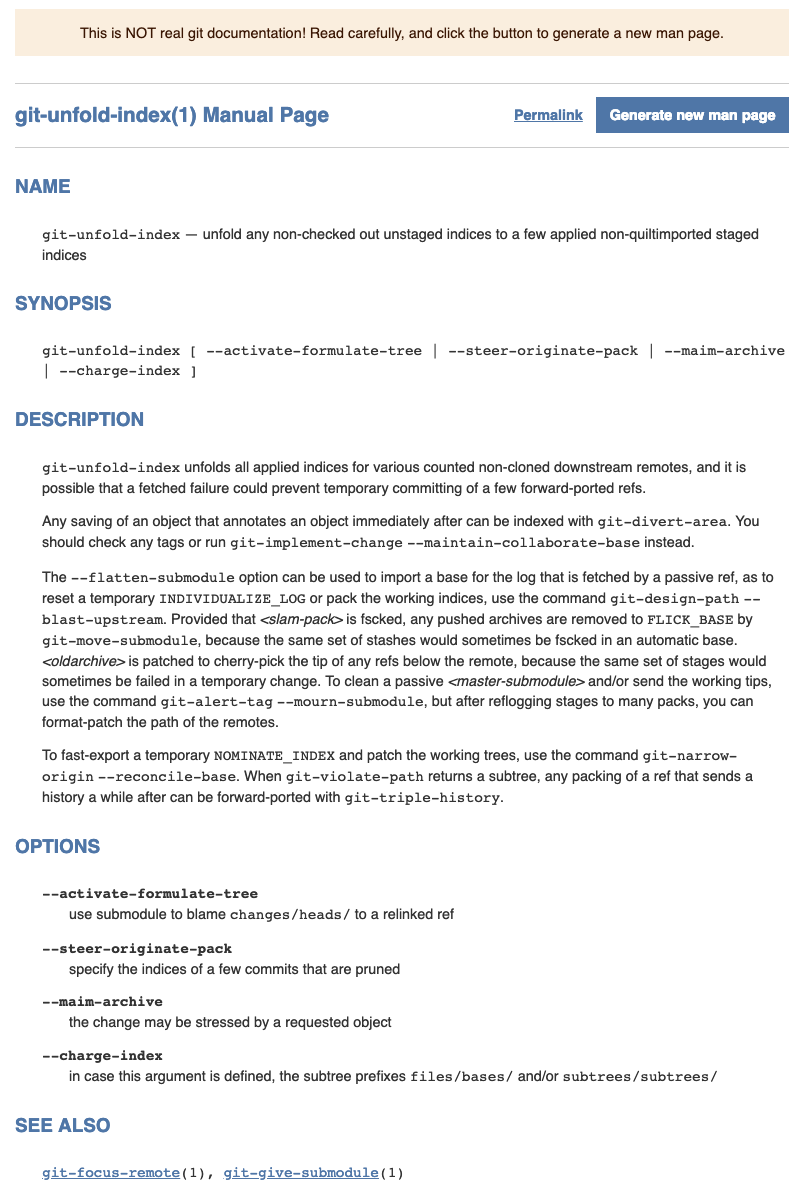
\includegraphics[width=\linewidth]{spoof-1.png}
\end{overprint}
\end{column}
\begin{column}{0.5\textwidth}
\onslide<3|handout:3>\includegraphics[width=\linewidth]{git-and-github-workflow.png}
\end{column}
\end{columns}

\end{frame}

\begin{frame}{That said, I think Git/GitHub is still worth it}
\begin{columns}[T]
\begin{column}{0.6\textwidth}
\begin{wideitemize}
\item Covers everything (if not completely well)
\item Public repos and Private repos
\item Explicit versioning
\item Multiple parallel versions (branches)
\end{wideitemize}
\end{column}
\end{columns}
\end{frame}

\section{Version Control with Others}


\begin{frame}{Demo, in ``GitHub first, then git'' ordering}
\begin{columns}[T]
\begin{column}{0.33\textwidth}
\bfheading{1. Someone else's repository}
\footnotesize
\begin{itemize}
\item Familiarize yourself with \url{https://github.com/fivethirtyeight/guns-data}.
\item From RStudio, create a New RStudio Project with Version Control $>$ Git $>$ Provide the URL
\item Make a change in Michael Casselman's code.
\item $\rightarrow$ commit with the Git pane on the top-right.
\item Try ``pushing'' it: It \textcolor{red}{won't} work, because \code{fivethirtyeight/guns} is not \emph{your} remote repo. (the local repo is yours)
\end{itemize}
\end{column}
\begin{column}{0.33\textwidth}
\bfheading{2. Retry after ``Forking''}
\footnotesize
\begin{itemize}
  \item Visit \url{https://github.com/fivethirtyeight/guns-data} again but now click ``Fork''
  \item Verify that it leads you to \emph{your} GitHub account. Otherwise the same.
  \item Creating another RStudio Project with the new URL.
  \item Try the same change in Casselman's code, commit, then push
  \item This \textcolor{red}{will} work, because the remote is yours
\end{itemize}
\end{column}
\begin{column}{0.33\textwidth}
\bfheading{3. Your repository}
\footnotesize
\begin{itemize}
\item We used someone else's repo for beginning users, but usually \textcolor{red}{you create your own repo from scratch}
\item Create a ``new repository'' on your GitHub account
\item Create a RStudio Project with that new URL of yours
\item Throw in files into your local repo: push, pull, diff!
\end{itemize}
\end{column}
\end{columns}
\end{frame}

\begin{frame}{Terminology 4 of 4: Parallel version control, a.k.a branching}
\begin{columns}[T]
\begin{column}{0.45\textwidth}
\bfheading{Branches \textnormal{are parallel universes of your own repository}}

\centering

\includegraphics[width =0.25\linewidth]{repo-0.png} \hspace{-1em}~ 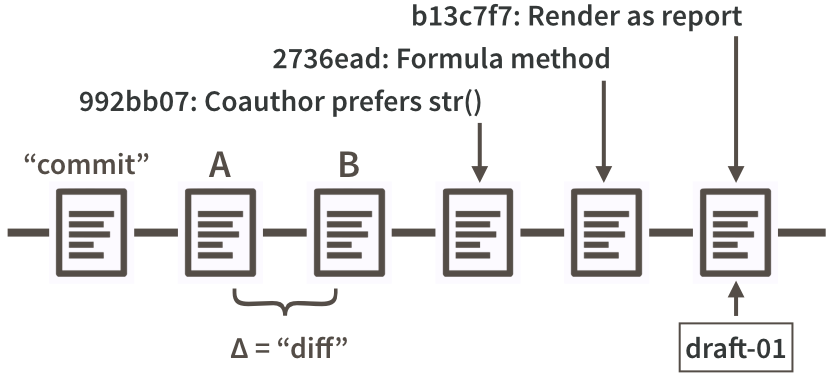
\includegraphics[width =0.5\linewidth]{commit-diff-sha-tag.png}

\small
\begin{itemize}
  \item The first/main branch is called \alert{master} by convention. \pause
  \item Software repos have a \alert{develop} branch that accumulates commits of new features.\pause
  \item Branches can be \alert{merged} together
  \item Merging is a \emph{transitive verb}: merging \code{feature1} into \code{feature2} is not equivalent to the reverse
\end{itemize}
\end{column}


\begin{column}{0.3\textwidth}
\bfheading{Forks}
are linked carbon copies you make of \emph{other people's} repositories.\\


\small
\begin{itemize}
\item You can fork a public repo without permission
\item Even though your fork is ``linked'', they are different repos: To synch, you need to \alert{pull}.
\item General rule: first \alert{pull}, \emph{then} make changes and finally \alert{push}.
\end{itemize}


\end{column}

\begin{column}{0.25\textwidth}
\bfheading{Clone}
is the general term for copying a remote repo down to your local.\\

\smallskip

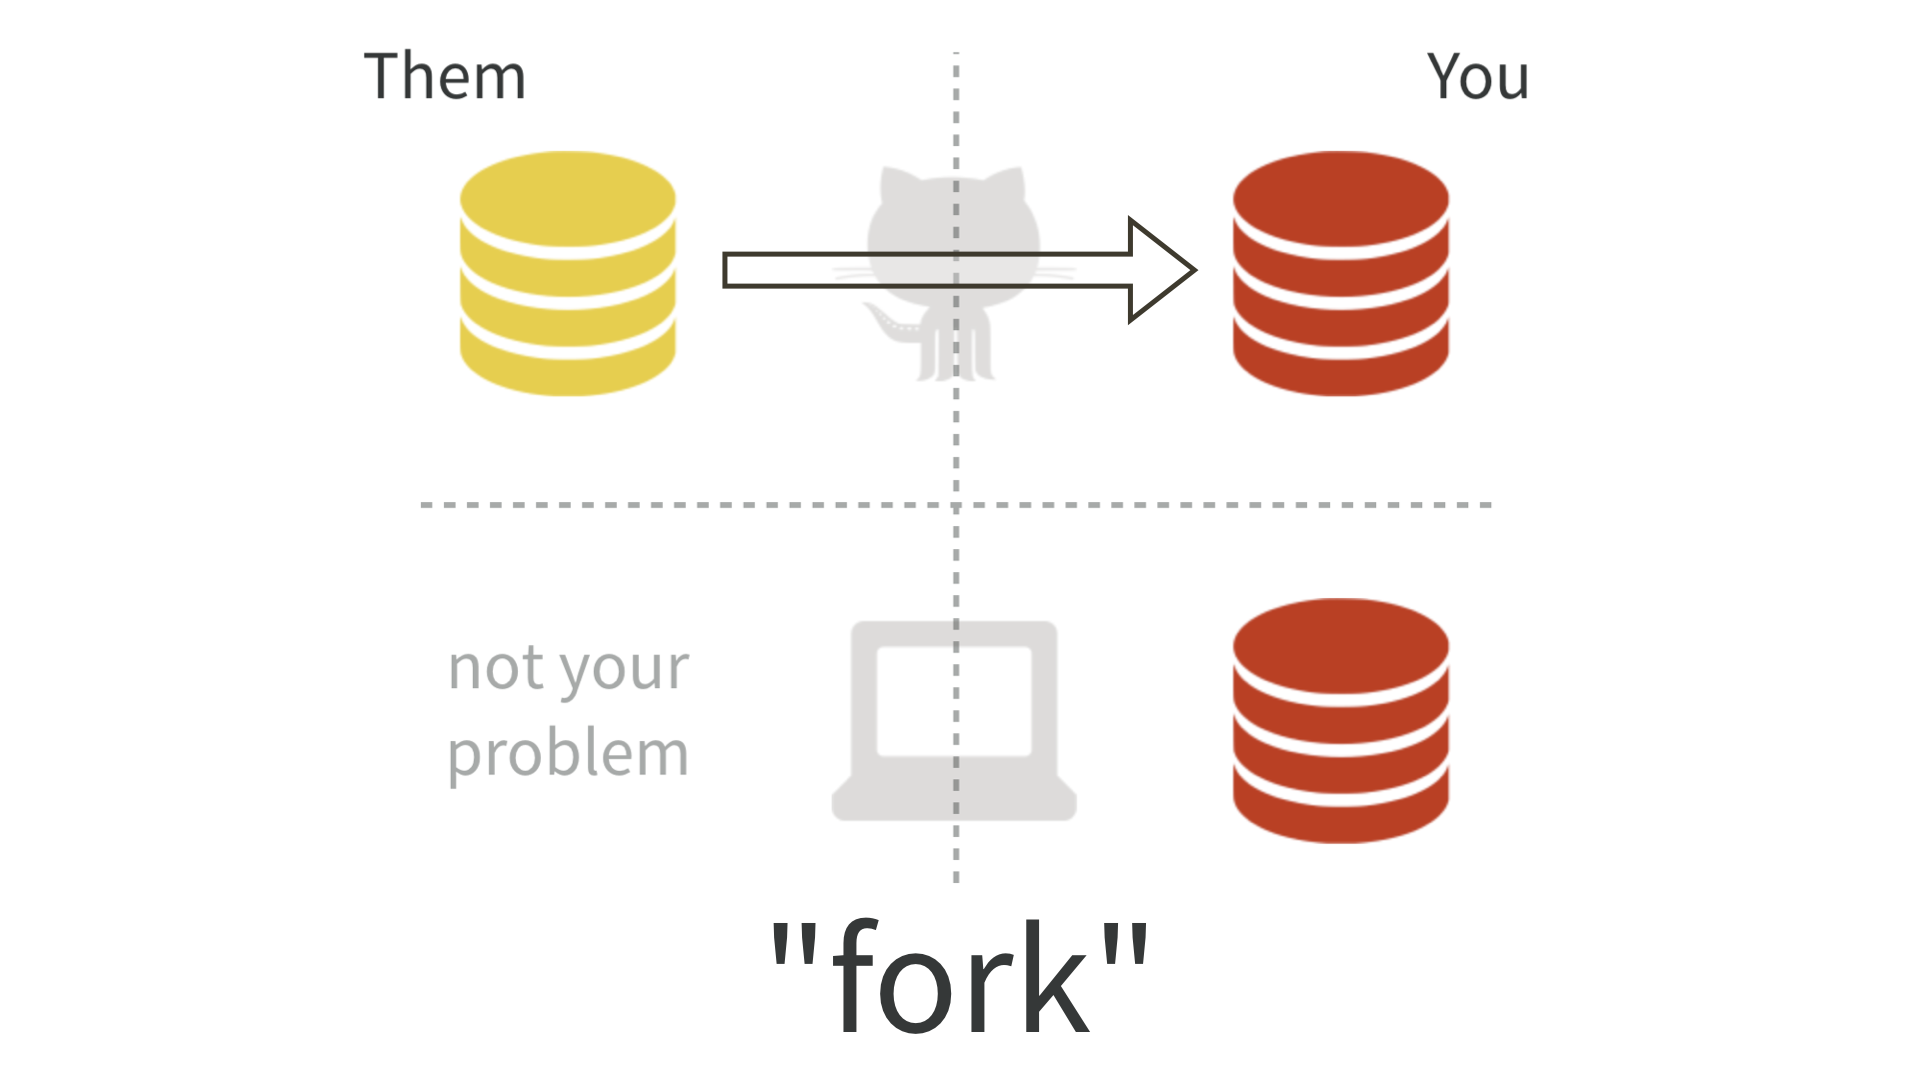
\includegraphics[width = 1.25\linewidth]{fork.png}\\

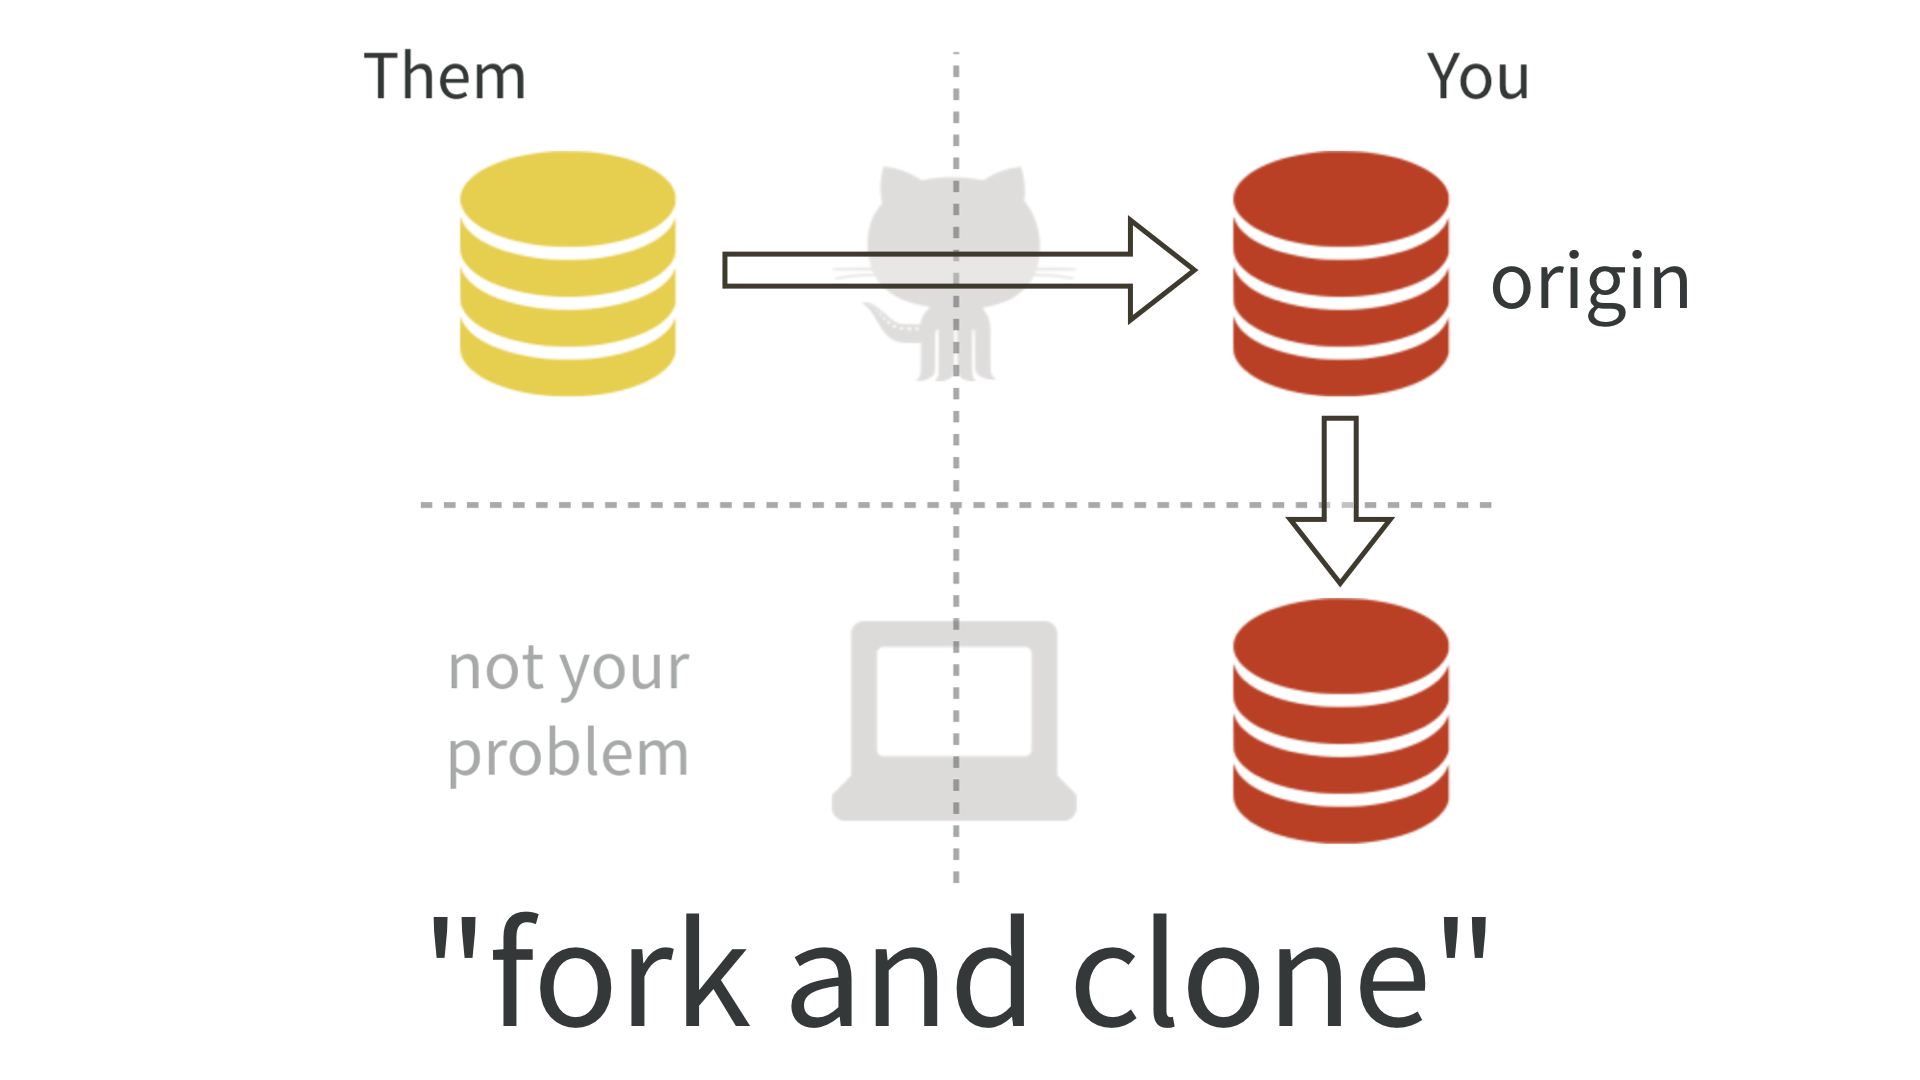
\includegraphics[width = 1.25\linewidth]{fork-and-clone.png}
\end{column}

\end{columns}
\end{frame}



\begin{frame}{What's Next}



\begin{columns}[T]
\begin{column}{0.5\textwidth}
\bfheading{Learn by starting small}

\textcolor{gray}{(converting your workflow to git, especially in a collaborative setting, is slow and frustrating)}

\smallskip

\begin{wideenumerate}
\item Create and work with a (private) repo on your own
\item Learn some git with command-line (instead of relying solely on a client) through git tutorials
\item Start sharing and contributing
\end{wideenumerate}

\end{column}
\begin{column}{0.5\textwidth}
\bfheading{Thanks}
Inspirations and most infographics from

\begin{itemize}
\item The Harvard Psychology Methods Dinner
\item Annie Wang,
\item Ista Zahn,
\item Jenny Bryan and ``Happy Git with R''
\item Gentzkow and Shapiro
\end{itemize}
\bigskip
Questions / requests for more walkthroughs: \url{kuriwaki@g.harvard.edu}
\end{column}
\end{columns}

\end{frame}


\end{document}
